%%%%
\documentclass[12pt,a4paper]{report}

% packages...
\usepackage[utf8]{inputenc}
\usepackage[english,italian]{babel}
\usepackage[hyphens]{url}
\usepackage{csquotes}
\usepackage{caption}
\usepackage{subcaption}
% Per generare il file PDF aderente alle specifiche PDF/A-1b. Verificarne poi la validità.
%\usepackage[a-1b]{pdfx}

\usepackage{hyperref}
\usepackage{graphicx}
\graphicspath{ {Img/} }
\usepackage{lipsum}% Per inserire testo a caso in attesa di realizzare i capitoli
\usepackage{listings}
\usepackage{epigraph} % per le frasi inizio capitolo
\usepackage{fancyhdr}
% \usepackage{refcheck}

\usepackage{pgfplots} 
\pgfplotsset{compat=1.18} 


\lstset{
	% 	language=bash
	frame=single,
	breaklines=true,
	postbreak=\raisebox{0ex}[0ex][0ex]{\ensuremath{\color{red}\hookrightarrow\space}},
	basicstyle=\ttfamily\footnotesize
}


%MyStyle
\renewcommand{\lstlistingname}{Code}

\definecolor{codegray}{rgb}{0.5,0.5,0.5}
\definecolor{codepurple}{rgb}{0.58,0,0.82}
\definecolor{backcolour}{rgb}{0.95,0.95,0.92}

\lstdefinestyle{Cstyle}{
    backgroundcolor=\color{backcolour},   
    keywordstyle=\color{blue},    
    numberstyle=\tiny\color{codegray},
    stringstyle=\color{codepurple},
    basicstyle=\ttfamily\footnotesize,
    breakatwhitespace=false,         
    breaklines=true,                 
    captionpos=b,                    
    keepspaces=true,                 
    numbers=left,                    
    numbersep=5pt,                  
    showspaces=false,                
    showstringspaces=false,
    showtabs=false,                  
    tabsize=2,
    frame = leftline
}

% RISC style
\lstdefinelanguage{Risc-v}
{
  alsoletter={.}, % allow dots in keywords
  alsodigit={0x}, % hex numbers are numbers too!
  morekeywords=[1]{ % instructions
    lb, lh, lw, lbu, lhu,
    sb, sh, sw,
    sll, slli, srl, srli, sra, srai,
    add, addi, sub, lui, auipc,addiw
    xor, xori, or, ori, and, andi,
    slt, slti, sltu, sltiu,
    beq, bne, blt, bge, bltu, bgeu,
    j, jr, jal, jalr, ret,
    scall, break, nop
  },
  morekeywords=[2]{ % sections of our code and other directives
    .align, .ascii, .asciiz, .byte, .data, .double, .extern,
    .float, .globl, .half, .kdata, .ktext, .set, .space, .text, .word
  },
  morekeywords=[3]{ % registers
    zero, ra, sp, gp, tp, s0, fp,
    t0, t1, t2, t3, t4, t5, t6,
    s1, s2, s3, s4, s5, s6, s7, s8, s9, s10, s11,
    a0, a1, a2, a3, a4, a5, a6, a7,
    ft0, ft1, ft2, ft3, ft4, ft5, ft6, ft7,
    fs0, fs1, fs2, fs3, fs4, fs5, fs6, fs7, fs8, fs9, fs10, fs11,
    fa0, fa1, fa2, fa3, fa4, fa5, fa6, fa7
  },
  morecomment=[l]{;},   % mark ; as line comment start
  morecomment=[l]{\#},  % as well as # (even though it is unconventional)
  morestring=[b]",      % mark " as string start/end
  morestring=[b]'       % also mark ' as string start/end
}

\lstset{
  % listings sonderzeichen (for german weirdness)
  literate={ö}{{\"o}}1
           {ä}{{\"a}}1
           {ü}{{\"u}}1,
  basicstyle=\tiny\ttfamily,                    % very small code
  breaklines=true,                              % break long lines
  commentstyle=\itshape\color{green!50!black},  % comments are green
  keywordstyle=[1]\color{blue!80!black},        % instructions are blue
  keywordstyle=[2]\color{orange!80!black},      % sections/other directives are orange
  keywordstyle=[3]\color{red!50!black},         % registers are red
  stringstyle=\color{mauve},                    % strings are from the telekom
  identifierstyle=\color{teal},                 % user declared addresses are teal
  frame=l,                                      % black line on the left side of code
  language=Risc-v,                   % all code is RISC-V
  tabsize=4,                                    % indent tabs with 4 spaces
  showstringspaces=false                        % do not replace spaces with weird underlines
}

%--- BIBIOGRAFIA
\usepackage[ backend=biber, style=alphabetic,
%citestyle=authoryear 
]{biblatex}

\addbibresource{Biblio.bib}
%---

\usepackage[textwidth=2cm, textsize=scriptsize,colorinlistoftodos]{todonotes}
\setlength {\marginparwidth }{2cm}
%\usepackage[disable]{todonotes}

%%%%%%%%%%%%%%%%%%%%%%%%%%%%%%%%%%%%%%%%%%%%%%%%%%%%%
\begin{document}

% Frontespizio
\begin{titlepage}
\begin{center}

\includegraphics[width=\textwidth]{Img/Logo.jpg}\\
{\large{\bf Corso di Laurea Informatica}}
\end{center}
\vspace{12mm}
\begin{center}
{\huge{\bf TITOLO}}\\
\vspace{4mm}
{\huge{\bf TITOLO}}\\
\vspace{4mm}
{\huge{\bf TITOLO}}\\
\end{center}
\vspace{12mm}
\begin{flushleft}
{\large{\bf Relatore:}}
{\large{Trentini Andrea}}\\
\vspace{4mm}
{\large{\bf Correlatore:}}
{\large{Carraturo Alexjan}}\\
\end{flushleft}
\vspace{12mm}
\begin{flushright}
{\large{\bf Tesi di Laurea di:}}
{\large{Bianchessi Mattia}}\\
{\large{\bf Matr. 931455}}\\
\end{flushright}
\vspace{4mm}
\begin{center}
{\large{\bf Anno Accademico xxxxxxxx}}
\end{center}
\end{titlepage}

%%%%%%%%%%
% TODO
%%%%%%%%%%
\listoftodos

%%%%%%%%
\chapter*{Introduzione}

Introduzione 

\todo{Introduzione \ldots}



\tableofcontents
\listoffigures
\listoftables
\lstlistoflistings

% o sections (dipende dal documentclass)

\chapter{RISC-V}
\todo{Rileggi/Correggi capitolo 1: RISC-V \ldots} 

% OUTLINE CH 1
%	definizione di computer \\
%	presentazione progetto \\
%	applicazione dalla nascita ad oggi  \\


\section{Dal codice alle istruzioni}
\begin{quote}
\textbf{Computer}  :
Apparecchio elettronico in grado di svolgere operazioni matematiche e logiche e di memorizzare informazioni a una velocità e in una quantità superiori a quelle di cui è comunemente capace il cervello umano; nelle sue componenti materiali ( hardware ) [..] e da un insieme di circuiti e di dispositivi sui quali si svolgono le funzioni di memoria, di elaborazione e di controllo, che avvengono grazie a programmi contenenti istruzioni ( software ); tali programmi sono basati su un sistema di computazione binario e sono scritti in vari linguaggi di programmazione;
\cite{DefinizioneComputer}
\end{quote}

Essere in grado di programmare significa essere in grado di scrivere un elenco di istruzioni interpretabili dal computer ed eseguibili. Il linguaggio scelto, che sia di alto livello o di basso livello,  deve essere tradotto in linguaggio macchina in questo modo puo essere eseguito dal nostro computer. Questo processo di chiama processo di compilazione mediante il quale il codice , scritto in linguaggio leggibile (human readeable) viene tradotto in codice sorgente che verrà poi sottoposto a determinate verifiche per poter essere approvato e trasformato in codice oggetto e poi file eseguibile.\\
All' interno del computer la componente che si occupa dell' esecuzione del codice è la CPU che,  leggendo le istruzioni tradotte dal codice (scritto e poi compilato) esegue delle operazioni specifiche. Come è normale pensare esistono differenti processori , differenti per frequenza di clock, memoria di cache, architettura interna  o tensione di alimentazione. Quindi il è necessario che il codice si chiaro e capibile per un determinato processore. \\

Un'Instruction Set Architecture (ISA) definisce il modello astratto di un computer ovvero come la CPU controlla hardware e software., specificando sia ciò che il processore è in grado di fare sia come viene fatto.

L'ISA fornisce l'unico modo attraverso il quale un utente è in grado di interagire con l'hardware. Può essere visto come un manuale del programmatore perché è la parte della macchina visibile al programmatore in linguaggio macchina,  allo scrittore del compilatore e al programmatore dell'applicazione.
L'ISA, inoltre, definisce i tipi di dati supportati, i registri, il modo in cui l'hardware gestisce la memoria principale. 

In informatica esistono due tipi popolari di architetture basate sul set di istruzioni. Si tratta di CISC (Complex Instruction Set Computing) e RISC (Reduced Instruction Set Computing).


Il primo approccio consiste in un ISA formata da un set di istruzioni in grado di eseguire operazioni complesse tramite una singola istruzione. Contrariamente il secondo approccio snellisce il set di istruzioni che porta ad avere un architettura più semplice e lineare.

\section{progetto RISC-V}
Il RISC-V è un progetto open source basato su un architettura di tipo RISC. Il progetto iniziato nel 2010 all'Università della California, Berkeley. In origine Prof. Krste Asanoviće e alcuni studenti (Yunsup Lee e Andrew Waterman) svilupparono un ISA per scopi didattici, inizialmente solo progettata e successivamente, dopo dei finanziamenti, prodotta. Il primo workshop risale al 2015 e al lancio il progetto contava 36 membri fondatori.

L'interesse per RISC-V non è dovuto all' architettura RISC o alla tecnologia rivoluzionaria ma il punto fondamentale è che RISC-V è uno standard libero che consente a chiunque di sviluppare in modo libero il proprio hardware per seguire il software.\\

Dopo il lancio il progetto fu studiato e utilizzato da molte realtà , come ad esempio in DARPA e Linux Foundation ,  e fu per questo che si fece conoscere molto presto al mondo.  Ora Il progetto RISC-V presenta numerose partnership con aziende e una community sparsa per tutto  il mondo.



\chapter{ISA RISC-V}

\todo{Rileggi/Correggi capitolo 2: ISA\ldots}
\section{ISA Overview}

L’istruction set architecture di RISC-V, originariamente pensato per supportare la ricerca e l’educazione, si è evoluto fino ad arrivare nell'industria. Alcuni punti focali dello sviluppo dell isa:
\begin{itemize}
	\item Un ISA open completamente disponibile per accademie e industrie
	\item Un ISA adatto per l'implementazione diretta per hardware, non una semplice emulazione
	\item Un ISA modulare estendibile e modificabile.
	\item Un ISA con supporto per implementazioni multicore e facilmente parallelizzabile per processi eterogenei
\end{itemize}


\subsection{Codifica Istruzione}
La base dell ISA di RISC-V è fissa di base a lunghezza 32-bit ma è modificabile a 16 o a 64 bit o altre lunghezze.  Ogni lunghezza  è codificata in una maniera chiara come mostrato in figura (Figura~\ref{Fig:lunghezza_Istruzioni}). Di base l’ISA è codificata in modo little-endian, (anche in questo caso  modificabile con altre tipologie di memorizzazione). 

\begin{figure}
	\centering
		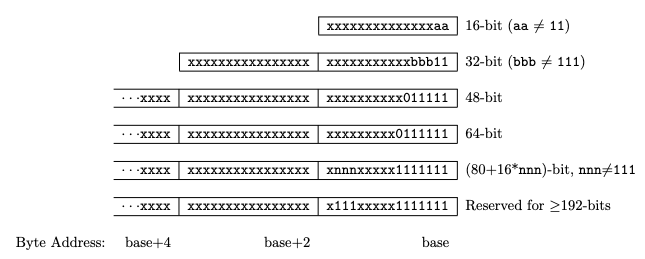
\includegraphics[width = \textwidth]{DiverseLunghezze.png}
		\caption{Lunghezza Istruzioni RISC-V}
		 \label{Fig:lunghezza_Istruzioni} 
\end{figure}


\subsection{Memorizzazione} 
Le istruzioni sono memorizzati in blocchi da 16.bit memorizzati in maniera little-endianess , non modificabile. Se ad esempio si ha un istruzione su 32 bit l’istruzione avviene divisa in due blocchi da 16-bit la parte più bassa dell istruzione viene memorizzata nel primo pacchetto e la parte più alta nel secondo pacchetto (Figura~ \ref{fig:memorizza_Istruzioni}). 

\begin{figure}
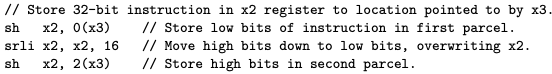
\includegraphics[width = \textwidth]{SomeLineCodeRISC.png}
\caption{Memorizza istruzioni} 
\label{fig:memorizza_Istruzioni} 
\end{figure}

\subsection{Cambio di flusso}
Si parla di eccezione quando una condizione non comune avviene a run time associata a un istruzione.
Si parla di trap quando verifica un trasferimento di controllo, da parte del trap handler, da un thread ad un altro. Si parla di interrupt quando la situazione imprevista è qualcosa di esterno.

\subsection{Nomi delle estensioni}
Nel manuale sono trattate diverse estensioni ognuna delle quali è identificata da una lettera 
M, A, F, D Q ,L, C, B, J ,T, P,V, N ogni estensione aggiunge delle istruzioni per un proprio fine. Oltre alle estensioni sono presentati 4 ISA di base RV32I, RV32E, RV64I, RV128I. Per ogni estensione e versione base sono indicate le versioni e se una di queste sono versioni definitive.
(Tabella 2.1)

\begin{table}
\centering
\begin{tabular}{|c|l|c|}
\hline
Base & Versione & Definitiva? \\
\hline
RV32I & 2.0 & S\\
RV32E & 1.9 & N\\
RV64I & 2.0 & S\\
RV128I & 1.7 & N\\
\hline
Estensione & Versione & Definitiva? \\
\hline
M & 2.0 & S\\
A & 2.0 & S\\
F & 2.0 & S\\
D & 2.0 & S\\
Q & 2.0 & S\\
L & 0.0 & N\\
C & 2.0 & S\\
B & 0.0 & N\\
J & 0.0 & N\\
T & 0.0 & N \\
P & 0.1 & N\\
V & 0.2 & N\\
N & 1.1 & N\\
\hline

\end{tabular}
	\caption{Tabella nomenclatura ISA RISC-V}
	\label{tab:nomenclaturaISA}
\end{table}

La tabella  \ref{tab:nomenclaturaISA}  presenta i set base RV32I, RV32E, RV64I, RV128I con le rispettive versioni. Ogni set presenta la casella 'Definitiva' che specifica se il set o l 'estensione è definitiva (S) o non lo è (N).

\section{ISA Base}
L'istruction set base ha la sigla di RV32I. 

\begin{quote}
RV32I was designed to be sufficient to form a compiler target and to support modern operating
system environments. The ISA was also designed to reduce the hardware required in a minimal implementation. RV32I contains 47 unique instructions, though a simple implementation
might cover the eight SCALL/SBREAK/CSRR* instructions with a single SYSTEM hardware
instruction that always traps and might be able to implement the FENCE and FENCE.I instructions as NOPs, reducing hardware instruction count to 38 total. RV32I can emulate almost
any other ISA extension (except the A extension, which requires additional hardware support for
atomicity).\cite{RISCV_ISA-DOC}
\end{quote}

\section{RV32I}
Il set è caratterizzato da registri a 32 bit. 31 dei quali registri general-purpose che memorizzano valori interi, identificati dalle sigle x1 - x31, il registro x0 è presente la costante 0.  Il termine XLEN rappresenta la lunghezza dei registri che in questo caso è 32.(Figura \ref{Fig:registri_arc_32})

\begin{figure}
\centering
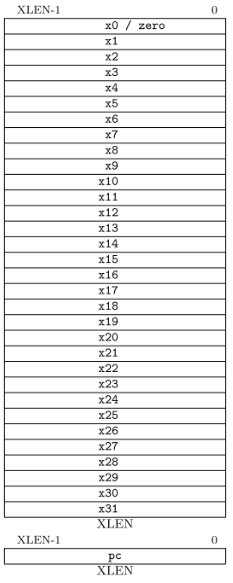
\includegraphics[scale= 0.7]{RegistriRV.png}
\caption{Registri architettura}
\label{Fig:registri_arc_32}
\end{figure}

\newpage

\subsection{Formato istruzioni }
Di base questo set presenta sei formati di istruzione (R/I/S/U/B/J) come mostrato in figura  (Figura 2.4).
Tutti i formati sono su 32 bit. In questi formati i registri source (rs1 e rs2) e il registro destination (rd) vengono mantenuti nelle stesse posizioni per semplificare la decodifica.


\begin{itemize}
	\item R:  Il formato presenta i due registri source e il registro destinazione
	\item I : Il formato presenta un registro source, una costante(immediato) e il registro destinazione.
	\item S : Il formato presenta una costante e due registri source.
	\item B : come il formato S. La costante su 12 bit rappresenta offsets di salto (branch) codificato sui propri bit in multipli di 2.
	\item U:come il formato I. I 20 bit del registro costante sono shiftati di 12 bit a sinistra. 
	\item J:come  il formato U. I 10 bit del registro costante sono shiftati solamente di 1 bit. 
\end{itemize}

\begin{figure}
	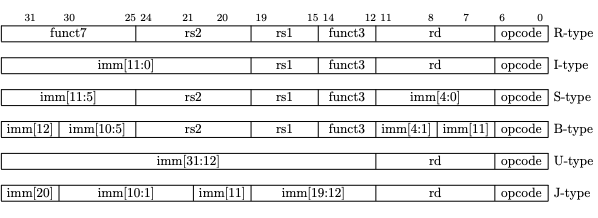
\includegraphics[width = \textwidth]{FormatiIstruzione.png}
	\caption{Formati istruzione RISC-V}
	\label{Fig:Formati_istruzioni_RV32I}
\end{figure}


\subsection{Istruzioni per computazione intera}
La maggior parte delle istruzioni che computano su valori interi opera su bit XLEN dei valori contenuti nei registri. Le istruzioni sono codificate e utilizzato il formato I (register-immediate) o il formato R (register-register). Il registro di destinazione.  La destinazione (rd) è la stessa per le istruzioni I che per le R.  Le istruzioni a computazione intera non causano eccezioni aritmetiche.\\



\subsection{Istruzioni registro-immediate}
Istruzioni di questo tipo utilizzano il formato I:
\begin{itemize}
	\item ADDI.  Viene aggiunta la costante nel registro immediato (12 bit) con estensione del segno per registrare rs1. L'overflow aritmetico viene ignorato e il risultato è semplicemente i bit bassi del risultato.
 \item NOP. Questa istruzione non modifica alcuno stato visibile all'utente, fatta eccezione per l'avanzamento del Program Counter (PC). L'istruzione è codificato come ADDI x0, x0, 0.
 \item SLTI.  Pone il valore 1 nel registro rd se il registro rs1 è minore del registro immediato con estensione del segno, altrimenti 0. rs1 viene anche trattato come un numero con segno.
\item SLTIU.  Come SLTI ma il valore in rs1 viene interpretato come privo di segno.
\item ANDI, ORI, XORI. Sono operazioni logiche che eseguono AND, OR e XOR bit per bit sul registro rs1 e il registro immediato a 12 bit con estensione del segno e posizionano il risultato in rd.
\end{itemize}

\begin{figure}
	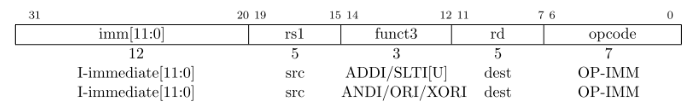
\includegraphics[width = \textwidth]{Istruzioni/Istruction1.png}
	\caption{Istruzioni registro-Immediato nel formato R}
	\label{Fig:Istruzioni_ri_formatoR}
\end{figure}


Le istruzioni in figura \ref{Fig:Istruzioni_ri_formatoI} sono nel formato I. Nel registro costante è presente un valore, codificato nei 5 bit del registro,  che è il valore di shift per il registro source. Lo shift a destra o a sinistra è a seconda del campo funct codificato su 3 bit.

\begin{itemize}
	\item  SLLI. shift logico a sinistra.
	\item SRLI. shift logica a destra.
	\item SRAI. shift aritmetico a destra.
\end{itemize}

\begin{figure}
	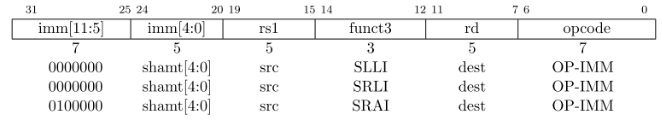
\includegraphics[width = \textwidth]{Istruzioni/Istruction2.png}
	\caption{Istruzioni registro-Immediato nel formato I}
	\label{Fig:Istruzioni_ri_formatoI}
\end{figure}

Le seguenti istruzioni utilizzano il formato U:
\begin{itemize}
\item  LUI. viene utilizzato per creare costanti a 32 bit utilizzando il formato U. Posiziona il valore U-immediato nei primi 20 bit del registro di destinazione rd, riempiendo i 12 bit più bassi con zeri.
\item AUIPC. viene utilizzato per creare indirizzi relativi al PC utilizzando il formato U.  Il risultato, come il caso precedente,  forma un offset di 32 bit dai 20 bit U-immediati, riempiendo i 12 bit più bassi con zeri, aggiunge questo offset al PC, quindi inserisce il risultato nel registro rd.
\end{itemize}

\begin{figure}
	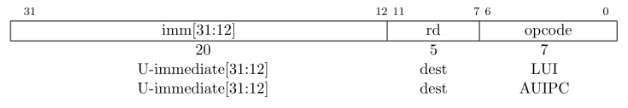
\includegraphics[width = \textwidth]{Istruzioni/Istruction3.png}
	\caption{Istruzioni registro-Immediato nel formato U}
	\label{Fig:Istruzioni_ri_formatoU}
\end{figure}


\subsection{Operazioni registro-registro}
Queste istruzioni utilizzano il formato R, gli operandi si trovano nei registri source e il risultato dell operazione è scritto nel registro destinazione. I campi funct7 e funct3 identificano il tipo di operazione.

\begin{itemize}
	\item ADD, SUB. Addizione e sottrazione. L'overflow è ignorato e il risultato è scritto nel registro destinazione.  
	\item SLT, SLTU. Operazione di comparazione tra i due registri rs1 e rs2, il risultato 1 (rs1 < rs2) o 0 è scritto nel registro destinazione. 
	\item SLL, SRL, SRA shift logici e aritmetici del valore codificato nei 5 bit piu bassi del registro rs2. Il valore da shiftare è nel registro rs1 e la direzione è identificata dal 6 bit di rs2. Il risultato è memorizzato nel registro rd.
\end{itemize}

\begin{figure}
	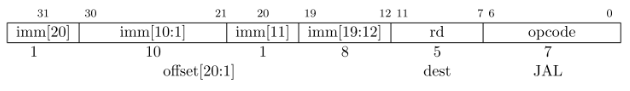
\includegraphics[width = \textwidth]{Istruzioni/Istruction4.png}
	\caption{Istruzioni registro-registro}
		\label{Fig:Istruzioni_rr}
\end{figure}

\subsection{Controllo del flusso}
RV32I presenta due tipi di trasferimento di controllo: salto incondizionato e condizionato.
\subsubsection{Incondizionato}
\begin{itemize}
	\item JAL. Usa  il formato J. Il campo immediato codifica numeri con segno in multipli di 2 byte.. The offset is sign-extended and added to the PC to form the jump target address. L'offset viene esteso con il segno e aggiunto al PC per formare l'indirizzo di destinazione del salto, l 'indirizzo di destinazione è memorizzato in rd.
	\item JALR. Usa il formato I.L'indirizzo di destinazione si ottiene sommando i 12 bit con segno I-immediate al registro rs1, quindi impostando a zero il bit meno significativo del risultato. L'indirizzo dell'istruzione successiva al salto (PC+4) viene scritto nel registro rd. Il registro x0 può essere utilizzato come destinazione se il risultato non è richiesto.
\end{itemize}
Entrambe le istruzioni possono generare dei disallineamenti se questo si verifica si verifica un eccezione.

\begin{figure}
	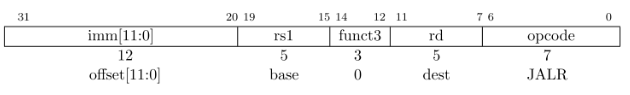
\includegraphics[width = \textwidth]{Istruzioni/Istruction5.png}
	\caption{Istruzioni per salto incondizionato}
	\label{Fig:Istruzioni_saltoIncondizionato}
\end{figure}

\subsubsection{Condizionato}
Tutte le istruzioni per il salto condizionato sono del formato B. Per calcolare l'indirizzo target viene utilizzata la cosante su i 12 bit che viene aggiunta al valore corrente di PC.
\begin{itemize}
	\item BQE, BNE. Salto eseguito se rs1 è uguale a rs2 nel primo caso,  diversi nel secondo.
	\item BLT, BLTU. Salto eseguito se rs1 è minore di rs2. Nel primo caso i due operandi vengono considerati con segno, nel secondo senza segno.
	\item BGE, BGEU.Salto eseguito se rs1 è maggiore o uguale di rs2. Nel primo caso i due operandi vengono considerati con segno, nel secondo senza segno.
	\item BGT, BGTU, BGT, BGTU.  Possiamo sintetizzarli come l 'inverso dei precedenti.
\end{itemize}
\begin{figure}
	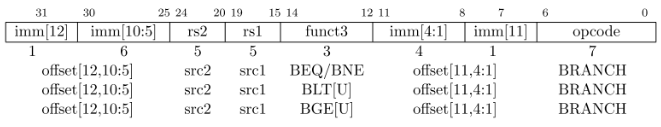
\includegraphics[width = \textwidth]{Istruzioni/Istruction6.png}
	\caption{Istruzioni per salto condizionato}
		\label{Fig:Istruzioni_saltoCondizionato}
\end{figure}

\subsection{Load e Store}
In RV32I  sono presenti diverse istruzione di load e store queste accedono  alla memoria mentre le istruzioni aritmetiche operano solo sui registri della CPU. Lo spazio fornito da RV32I è uno spazio di indirizzi  a 32 bit con in modalità little-endian.  Le istruzioni di load e store con destinazione il registro x0 sollevano un eccezione, anche se il valore poi verra scartato.

Le istruzioni di load e store trasferiscono il valore tra i registri e la memoria. Le istruzioni di load utilizzano il formato I mentre il formato per le istruzioni store è quello S. L'indirizzo del byte effettivo si ottiene aggiungendo il registro rs1 all'offset a 12 bit con estensione del segno. 
Store (vedi Figura ). Load (vedi Figura ).

\begin{itemize}
	\item LW, LH, LHU, LB, LBU. LW carica il valore codificato su 32 bit dalla memoria in rd. LHU 
carica un valore a 16 bit dalla memoria, quindi il segno si estende a 32 bit prima di archiviarlo in rd, mentre LHU fa lo stesso ma esegue un'estensione zero a 32 bit. LB e LBU sono definiti in modo analogo a LH e LHU ma per valori a 8 bit.
	\item SW, SH, SB. Memorizzano rispettivamente valori a 32 bit, 16 bit e 8 bit dai bit bassi del registro rs2 alla memoria.
\end{itemize}

L'ISA di base supporta accessi disallineati per i dati, ma questo potrebbe essere molto inefficienti e lento, a seconda dell'implementazione. Per questo motivo,vengono garantiti accessi a sezioni allineate solo per l'esecuzione atomica.

\begin{figure}
	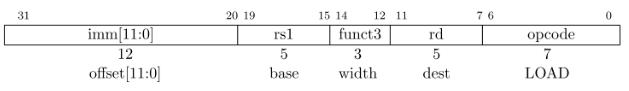
\includegraphics[width = \textwidth]{Istruzioni/Istruction7.png}
	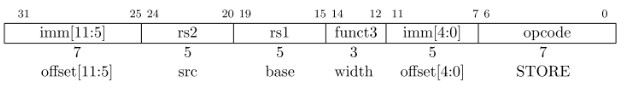
\includegraphics[width = \textwidth]{Istruzioni/Istruction8.png}
	\caption{Istruzioni load e store}
	\label{Fig:Istruzioni_LS}
\end{figure}

\subsection{Controllo e i registri di stato}
Le informazioni di sistema sono memorizzate in registri speciali chiamati Control Status Registers (CSR). Questi registri di solito memorizzano informazioni sull'istruzione precedente eseguita e sulla modalità operativa. RV32I consente di accedere a quei registri con formato di istruzione di tipo I. In base all'implementazione, queste istruzioni possono richiedere l'esecuzione di un accesso privilegiato.

\subsubsection{Istruzioni CSR}
Tutte le istruzioni:
\begin{itemize}
	\item CSRRW. ("Atomic Read/Write CSR"),questa istruzione scambia in modo atomico i valori nei CSR e nei registri interi. CSRRW legge il vecchio valore del CSR, estende a zero il valore a 32 bit, quindi lo scrive nel registro intero rd. Il valore iniziale in rs1 viene scritto nel CSR. Se rd=x0, l'istruzione non dovrebbe leggere il CSR.
	\item CSRRS. ("Atomic Read and Set Bits in CSR"),questa istruzione legge il valore del CSR, estende a zero il valore a 32 bit e lo scrive nel registro intero rd. Il valore iniziale nel registro intero rs1 viene trattato come una maschera di bit che specifica le posizioni di bit da impostare nel CSR. Qualsiasi bit alto in rs1 farà sì che il bit corrispondente venga impostato nel CSR, se quel bit CSR è scrivibile. Gli altri bit nella CSR non sono interessati. Come per l'istruzione precedente, se rs1=x0, l'istruzione non scriverà affatto nel CSR.
	\item CSRRC.("Atomic Read and Clear Bits in CSR"), questa istruzione legge il valore del CSR, estende a zero il valore a 32 bit e lo scrive nel registro intero rd. Il valore iniziale nel registro intero rs1 viene trattato come una maschera di bit che specifica le posizioni di bit da cancellare nel CSR. Qualsiasi bit alto in rs1 provocherà la cancellazione del bit corrispondente nel CSR, se quel bit CSR è scrivibile. Gli altri bit nella CSR non vengono modificati. Se rs1=x0, l'istruzione non scriverà affatto nel CSR.
	\item CSRRWI, CSRRSI, CSRRCI. Sono varianti delle precedenti e sono simili tranne per il fatto che aggiornano il CSR utilizzando un valore a 32 bit ottenuto estendendo a zero un campo immediato senza segno (uimm[4:0]) a 5 bit codificato nel campo rs1 invece di un campo valore da un registro intero.
\end{itemize}

\begin{figure}
	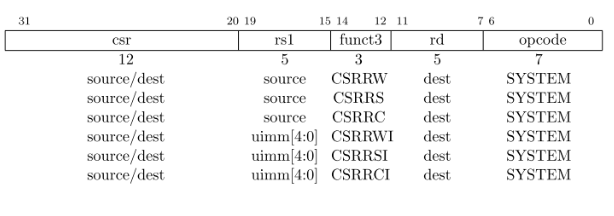
\includegraphics[width = \textwidth]{Istruzioni/Istruction9.png}
	\caption{Istruzioni CSR}
	\label{Fig:IstruzioniCSR}
\end{figure}

\subsubsection{Timer e counter}
RV32I fornisce una serie di contatori a livello utente di sola lettura a 64 bit, che sono mappati nello spazio degli indirizzi CSR a 12 bit e accessibili in parti a 32 bit utilizzando le istruzioni CSRRS.
\begin{itemize}
	\item RDCYCLE[H]. La pseudo-istruzione RDCYCLE legge i 32 bit bassi del ciclo CSR che contiene un conteggio del numero di cicli di clock eseguiti dal core del processore che è in esecuzione da un'ora di inizio arbitraria nel passato. RDCYCLEH è un'istruzione solo RV32I che legge i bit 63–32 dello stesso contatore di cicli. (La frequenza del ciclo (cicli/secondo) del contatore dipendono solamente dall'implementazione.)
	\item RDTIME[H]. La pseudo-istruzione RDTIME legge i 32 bit bassi del CSR temporale, che conta il tempo reale trascorso da un'ora di inizio arbitraria nel passato. RDTIMEH è un'istruzione solo RV32I che legge i bit 63–32 dello stesso contatore in tempo reale. (L'ambiente di esecuzione fornisce i dati per determinare il periodo del contatore in tempo reale (secondi/tick).)
	\item  RDINSTRET[H]. Questa pseudo-istruzione legge i 32 bit bassi della CSR INSTRET, che conta il numero di istruzioni eseguite da un punto di inizio arbitrario in passato. RDINSTRETH è un'istruzione esclusiva per RV32I che legge i bit 63–32 dello stesso contatore di istruzioni.
\end{itemize}

\begin{figure}
	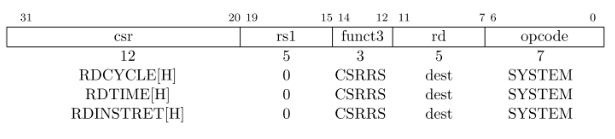
\includegraphics[width = \textwidth]{Istruzioni/Istruction10.png}
	\caption{Time e counter}
	\label{Fig:Istruzioni_TimerCounter}
\end{figure}

\subsection{Pseudo-istruzioni}
Nel manuale dell ISA di RISC-V sono presentate anche le pseudo-istruzioni di base. Le pseudo-istruzioni presentate mostrano che la maggior parte delle istruzioni ha una traduzione 1 a 1 con istruzioni regolari. Con l'inserimento si da la possibilità di avere un codice assembly molto piu comprensibile e intuitivo, naturalmente la compattezza del codice solo in alcuni casi, con le istruzioni standard, in quanto solo qualche pseudo-istruzione viene tradotta con piu istruzioni regolari.Questo comporta , per un programmatore RISC-V, a non dover configurare delle pseudo-istruzioni di utilità. Comunque è possibile costumizzare l'ISA inserendo altre pseudo.istruzioni.

\section{Alcune estensioni}
\subsection{Estensione M}
I lettori più attenti si saranno di certo accorti che tra le istruzioni presentate nel set base non è presente nessuna operazione di moltiplicazione. Certamente è possibile implementare questa operazione utilizzando addizioni in loop ma è piu macchinoso di scrivere un unica istruzione. L'estensione denominata "M" introduce le istruzioni standard di moltiplicazione e divisione di interi, che moltiplicano o dividono i valori contenuti in due registri di interi. Le istruzioni introdotte da questa estensione sono:
\begin{itemize}
\item MUL, MULH, MULHU, MULHSU.  Operazione di moltiplicazione. L'operazione MUL moltiplica gli operandi su 32 bit a posizionano i 32 bit meno significativi new registro destinazione. Le altre 3 invece operano su operandi considerati entrembi con segno, entrambi senza segno e rs1 con segno e rs2 senza segno , rispettivamente, e il risultato sono i 32 bit piu significativi che vengono memorizzati nel registro destinazione.
\item DIV, DIVU. Calcolano il risultato della divisione con segno e senza segno degli interi e i registri corrispondenti.
\item REM, REMU. Calcolano il resto della divisione con segno e senza segno degli interi e i registri corrispondenti.
\end{itemize}
\begin{figure}
	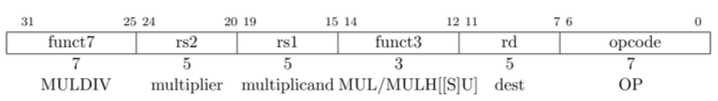
\includegraphics[width = \textwidth]{Istruzioni/IstruzioniM/Istruction1_M.png}
	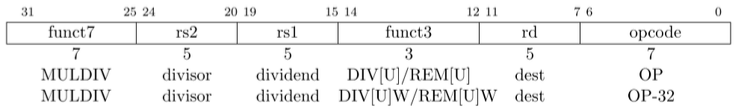
\includegraphics[width = \textwidth]{Istruzioni/IstruzioniM/Istruction2_M.png}
	\caption{Istruzioni moltiplicazione e divisione dell estensione M}
	\label{Fig:IstruzioniM}
\end{figure}



\subsection{Estensione F}
Questa estensione provvede a fornire delle operazioni Single-Precision e Floating-Point.
L'estensione F prevede 32 registri a virgola mobile, f0–f31 e un registro di controllo e di stato a virgola mobile (FCSR), che contiene la modalità operativa e lo stato di eccezione dell'unità a virgola mobile.  mostra il file di registro a virgola mobile e l'FCSR. Il termine FLEN descrive la larghezza dei registri a virgola mobile nel RISC-V ISA. FLEN=32 corrisponde alla lunghezza per l'estensione in virgola mobile a precisione singola.
Con questa estensione ci sono le operazioni:
\begin{itemize}
\item FADD. Calcola l'addizione
\item FSUB. Calcola la sottrazione
\item FMUL. Calcola la sottrazione
\item FDIV. Calcola la divisione
\item FMIN. Scrive il minimo tra rs1 e rs2 in rd
\item FMAX. Scrive il massimo tra rs1 e rs2 in rd
\item FSQRT. Calcola la radice.
\end{itemize}

\begin{figure}
	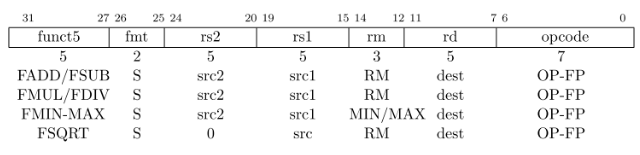
\includegraphics[width = \textwidth]{Istruzioni/IstruzioniF/Istruction1_F.png}
	\caption{Istruzioni Single-Precision registro-register nel formato R }
	\label{Fig:Istruzioni_SP-FormatoR}
\end{figure}

Oltre a queste operazioni semplici l'estensione presenta anche altre operazioni.
\begin{itemize}
	\item FMADD rs1×rs2+rs3.
	\item FMSUB rs1×rs2-rs3.
	\item FNMSUB -rs1×rs2+rs3. 
	\item FNMADDrs1×rs2-rs3.

\end{itemize}

\begin{figure}
	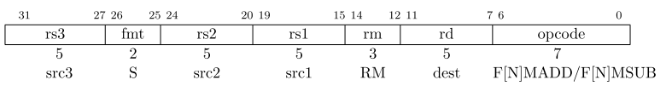
\includegraphics[width = \textwidth]{Istruzioni/IstruzioniF/Istruction2_F.png}
	\caption{Istruzioni Single-Precision registro-register in un formato speciale }
	\label{Fig:Istruzioni_SP-Special}
\end{figure}

Per distinguere le operazini in single-Precision e in double-Precisione l'estensione prevede un ulteriore lettera identificativa all nome dell istruzione. A livello di codifica il campo fmt 2 bit identifica la codifica del numero floating-point.  (Tabella 2.2)Guardando del codice ci permette di capire se parliamo di un n-esima Precisione  e ci fa capire la lunghezza dei registri utilizzati.


\begin{table}
\centering
\begin{tabular}{ |c|c|c| }
\hline
fmt & Lettera & Significato \\
\hline
00 & S & 32-bit single precision \\
\hline
01 & D & 64-bit double-precision\\
\hline
10 & \_ & riservato \\
\hline
11 & Q & 128-bit quad-precision \\
\hline
\end{tabular}
\caption{Campo fmt}
\label{Tab:Tabella_significato_fmt}
\end{table}


Oltre alle istruzioni aritmetiche sono introdotte anche le apposite istruzioni di load e store, move e di comparazione che sono molto simili come logica all ISA base. Ogni istruzione puo sollevare un eccezione di Invalid Operation se almeno un operatore non rispetta il tipo specificato.
Come ultima cosa con questa estensione è introdotta un istruzione:
\begin{itemize}
	\item FCLASS.S. Questa istruzione esamina il valore nel registro a virgola mobile rs1 e scrive nel registro intero rd una maschera a 10 bit che indica la classe del numero a virgola mobile. Il formato della maschera è descritto nella Tabella 2.3. Il bit corrispondente in rd sarà impostato se la proprietà è true e clear in caso contrario. Tutti gli altri bit in rd vengono cancellati. Si noti che verrà impostato esattamente un bit in rd.
\end{itemize}

\begin{table}
	\centering
	\begin{tabular}{ | c | c |}
	\hline
	Valore & Significato \\ 
	\hline
	0 & rs1 is  $- \infty$. \\
	1 & rs1 is a negative normal number.\\	
	2 & rs1 is a negative subnormal number.\\	
	3 & rs1 is - 0 .\\	
	4 & rs1 is $+0$.\\	
	5 & rs1 is a positive subnormal number.\\	
	6 & rs1 is a positive normal number.\\	
	7 & rs1 is $\infty$.\\	
	8 & rs1 is a signaling NaN.\\	
	9 &rs1 is a quiet NaN.\\ 
	\hline
	\end{tabular}
	\caption{Formato del risultato di FCLASS}
	\label{Tab:Formato_FCLASS}
\end{table}



\subsection{E per Embedded}
RV32E Isa sviluppato per dispositivi Embedded. La differenza principale sta nel avere la meta dei registri x0-x15 (x0 mantiene sempre la costante 0) al posto dei 32 di RV32I. Le istruzioni utilizzabili sono le istruzioni che utilizzano i registri ammissibili mentre le istruzioni che richiedono i registri x16-x31 risultano illegali e , se utilizzate, sollevano eccezioni. Anche con RV32E può essere estensibile con alcune estensioni standard.

\section{ Altri Set}
Esistono altri set che aumentano i bit utilizzati dai registri come RV64I e RV128I. Tutto cio che è stato detto è valido anche per queste con un piccolo accorgimento che l'estensione E ed F sollevano eccezioni di operazioni non valide.\\
Esistono altre estensioni come l'estensione per le istruzioni atomiche "A". Essa  contiene istruzioni che leggono-modificano-scrivono in modo atomico dalla e alla memoria per supportare la sincronizzazione tra
più thread RISC-V in esecuzione nello stesso spazio di memoria. Le due forme di istruzione atomica
vengono fornite istruzioni apposite per supportare la sincronizzazione. Entrambi i tipi di istruzione atomica supportano vari ordini di coerenza della memoria, inclusi
semantica disordinata, di acquisizione, di rilascio e sequenzialmente coerente. Queste istruzioni consentono a RISC-V di supportare la coerenza della memoria.\\
E infine è presente un estensione che comprime il codice. Questa è chiamata "C". Con questa estensione l'istruzione viene ridotta a 16 bit e compressa. L'estensione C può essere aggiunta a qualsiasi base
ISA (RV32, RV64, RV128) e usiamo il termine generico "RVC" per coprire ognuno di questi. Tipicamente,
Il 50\%–60\% delle istruzioni RISC-V in un programma può essere sostituito con istruzioni RVC, risultanti
con una riduzione della dimensione del codice del 25\%–30\%.


Sul documento che propone RISC-V sul proprio ISA vengono anche impostate le linee guida per fare delle proprie estensioni.



\chapter{Compilatori}

\todo{Rileggi/Correggi capitolo 3: Compilatore\ldots}

\section{Descrizione}
Un compilatore è un programma che trasforma il codice sorgente scritto in un determinato linguaggio di programmazione,  in un altro linguaggio informatico (codice target). Il motivo più comune per trasformare il codice sorgente è creare un programma eseguibile. Il linguaggio attraversa diverse fasi prima di diventare il codice target. La prima attivita è l' analisi lessicale dove il programma viene analizzato parola per parola e genera dei token. La seconda attivita è l analisi sintattica dove viene controllata la correttezza formale del programma. In questa fase i token precedentemente generati vengono analizzati e utilizzati per generare una struttura ad albero che nella fase di analisi semantica viene analizzato per verificare la correttezza delle espressioni scritte.  Infine viene generato il codice target.  Alcuni compilatori prevedono un ulteriore fase la fase di ottimizzazione dove il codice viene ottimizzato 

\begin{figure}
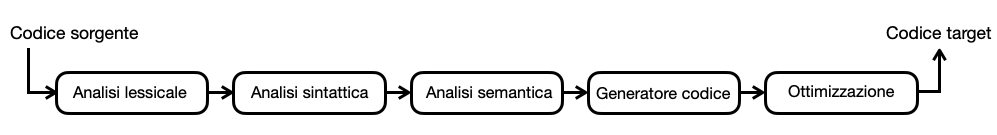
\includegraphics[width = \textwidth]{SchemaCompilatore.png}
\caption{Schema meccanismo di compilazione}
\label{Fig:MeccanismoCompilazione}
\end{figure}


Qualsiasi programma scritto in un linguaggio di programmazione di alto livello deve essere tradotto in codice oggetto prima di poter essere eseguito, quindi tutti i programmatori che utilizzano tale linguaggio utilizzano un compilatore o un interprete. I miglioramenti a un compilatore possono portare a un gran numero di funzionalità migliorate nei programmi eseguibili.

\section{Storia}
Il primo compilatore teorico fu pensato da Corrado Böhm che nel 1951 che lo sviluppò per la sua tesi di dottorato . Il primo compilatore implementato è stato scritto da Grace Hopper , coniando il termine "compilatore". Il primo compilatore , chiamato sistema A-0,  funzionava come caricatore o linker , non come i moderni compilatori. E' importante menzionare che una versione successiva (la versione A-2 datata 1953)fu il primo software libero e open source della storia dell'informatica. \\

Il primo compilatore ALGOL 58 fu completato alla fine del 1958 da Friedrich L. Bauer , Hermann Bottenbruch, Heinz Rutishauser e Klaus Samelson per il computer Z22 . 
Nel 1960, un compilatore Fortran esteso, ALTAC, era disponibile sulla Philco 2000, quindi è probabile che un programma Fortran sia stato compilato per le architetture di computer IBM e Philco a metà del 1960.  Il primo linguaggio di alto livello multipiattaforma noto è stato COBOL. 

Come qualsiasi altro software, ci sono vantaggi nell'implementare un compilatore in un linguaggio di alto livello. In particolare, un compilatore può essere self-hosted , ovvero scritto nel linguaggio di programmazione che compila. Il sopracitato compilatore di Böhm è un compilatore self-hosted. Il suo compilatore, oltre ad essere completo, fu il primo definito con il proprio linguaggio.
Oltre a quel compilatore possiamo citare il Navy Electronics Laboratory International ALGOL Compiler (NELIAC) o il Lisp.\\

Come durante una comunicazione verbale anche i programmi hanno una propria grammatica con regole queste vengono analizzate da un parser, generato da un generatore, ha lo scopo di analizzare come è scritto il programma e generare i token associati. Un primo progetto risale al 1960 come progetto dell università di Università di Manchester, non è da considerare un compilatore moderno ma un buon punto per la costruzione e per l ideazione del sistema Unix nel 1969 da parte di Ken Thompson.\\

\section{Cross-compilazione}
\label{Sec:Cross}
Un compilatore incrociato è un compilatore in grado di creare codice eseguibile per una piattaforma diversa da quella su cui è in esecuzione il compilatore. Ad esempio, un compilatore che viene eseguito su un PC ma genera codice che viene eseguito su uno smartphone Android è un compilatore incrociato.

Un compilatore incrociato è utile per compilare codice per più piattaforme da un host di sviluppo. La compilazione diretta sulla piattaforma di destinazione potrebbe non essere fattibile, ad esempio su sistemi embedded con risorse informatiche limitate.

\section{Compilatori moderni}
Nel ecosistema dei compilatori moderni i piu famosi sono: GCC e CLANG.
Il primo GCC (GNU Compiler Collection) è un compilatore multipiattaforma creato nel 1987 da Richard Stallman. Oggi GCC viene sviluppato da programmatori da ogni parte del mondo ed è stato portato su più tipi di processori e sistemi operativi. GCC è il compilatore ufficiale di GNU e usato per lo sviluppo di altri sistemi operativi(macOS, DOS).
Nato per il linguaggio C,  oggi di vari front end per altri linguaggi, tra cui Java, C++, Objective C, e vari back-end   in grado di generare linguaggi macchina per varie architetture, come ad esempio x86,, ARM.\\

Il secondo, piu giovane, nato nel 2005 da Apple Inc. l'inizio dello sviluppo è dovuto a esigenze di avere un compilatore di casa Apple ottimizzato per dispositivi Apple. 
Il progetto LLVM originariamente intendeva utilizzare il front-end di GCC. Il codice sorgente di GCC, tuttavia, è grande e alquanto ingombrante; come ha affermato uno sviluppatore GCC di lunga data riferendosi a LLVM, 

\begin{center}
Trying to make the hippo dance is not really a lot of fun\\
 \begin{footnotesize}
 	Cercare di far ballare l'ippopotamo non è davvero molto divertente.
 \end{footnotesize}
 	
\end{center}

Inoltre, il software Apple utilizza Objective-C, che è una priorità bassa per gli sviluppatori GCC. Pertanto, GCC non si integra perfettamente nell'ambiente di sviluppo integrato (IDE) di Apple. Infine, il contratto di licenza di GCC, la GNU General Public License (GPL) V3, richiede agli sviluppatori che distribuiscono estensioni o versioni modificate di GCC di rendere disponibile il loro codice sorgente, ma la licenza software permissiva di LLVM è priva di tale impedimento.Alla fine, Apple ha scelto di sviluppare Clang, un nuovo front-end del compilatore che supporta C, Objective-C e C++. Nel luglio 2007 il progetto ha ricevuto l'approvazione per diventare open-source.


\section{Un buon compilatore}
I processori moderni hanno tutti pipeline superscalari e lunghe e strutture interne complesse e supportano unità di estensione vettoriale. Inoltre, gli standard dei moderni linguaggi avanzati astraggono costantemente i dettagli dell'hardware e delle strutture dati sottostanti per generare codice generale più logico e matematico, invece di istruzioni operative specifiche e percorsi di accesso alla memoria. Gli standard dei linguaggi, come C++, si fanno  sempre più espressivi e astratti. Una maggiore espressività aumenta l'onere del compilatore di generare un buon codice assembly dalle complesse strutture compilate dai programmatori. Il compilatore deve essere più intelligente e lavorare di più per massimizzare le prestazioni utilizzando il codice. Non tutti i compilatori possono farlo. Quando si seleziona un compilatore,  è necessario considerare se lo stesso segmento di codice può generare comandi assembly più efficienti con uno e l'altro compilatore.
Oltre a generare programmi eseguibili ad alte prestazioni, i compilatori moderni devono anche avere prestazioni elevate. Un progetto software di grandi dimensioni  può contenere da centinaia a migliaia di singole unità di traduzione. Ogni unità di traduzione può contenere migliaia di righe di codice. 
In termini di estensione del linguaggio, i moderni sistemi informatici con più kernel, capacità di elaborazione vettoriale e acceleratori forniscono capacità superiori alle capacità naturali dei comuni linguaggi di programmazione. Pertanto, specifici framework HPC (High Performance Computing), come OpenMP e OpenACC, per poter colmare questa lacuna. Questi framework forniscono API (Application Program Interface) che i programmatori possono utilizzare per esprimere il parallelismo nel codice.. Pertanto, i compilatori devono stare al passo con lo sviluppo degli standard di estensione del linguaggio.

In conclusione, un buon compilatore ci permette di concentrarci sul processo di programmazione, piuttosto che combatterne le carenze. Può supportare gli standard linguistici più recenti, generare comandi ottimizzati dal codice più astratto e compilare il codice sorgente in meno tempo.



\section{CLANG e GCC}
Clang è compatibile con GCC. Clang è un sostituto di GCC. Ma detta cosi ci si potrebbe chiedere perche usare uno o l 'altro. Analizziamo un po piu in dettaglio i due compilatori.
Gli sviluppatori di Clang mirano a ridurre l'ingombro di memoria e aumentare la velocità di compilazione rispetto ai compilatori concorrenti, come GCC. Nell'ottobre 2007 furono eseguiti dei test comparativi che portarono dei primi risultati notevoli, Clang ha compilato le librerie Carbon a una velocità doppia rispetto a GCC, utilizzando circa un sesto di memoria e spazio su disco di GCC. Con lo sviluppo di Clang e GCC il primo compila ancora costantemente più velocemente di GCC Tuttavia, entro il 2019, Clang è significativamente più lento nella compilazione del kernel Linux rispetto a GCC, pur rimanendo leggermente più veloce nella compilazione di LLVM.\\
Sebbene Clang sia stato storicamente più veloce di GCC nella compilazione, la qualità dell'output è rimasta indietro. A partire dal 2014, le prestazioni dei programmi compilati da Clang sono rimaste indietro rispetto alle prestazioni del programma compilato da GCC, a volte per fattori importanti (fino a 5x), replicando i precedenti rapporti di prestazioni più lente. Entrambi i compilatori si sono evoluti per aumentare le loro prestazioni da allora, con la riduzione del divario:

I confronti nel novembre 2016 tra GCC 4.8.2 e clang 3.4, su un numerosi file di test, mostrano che GCC supera il clang di circa il 17\% su un codice sorgente ben ottimizzato. I risultati dei test sono specifici del codice e il codice sorgente C non ottimizzato può invertire tali differenze. I due compilatori sembrano quindi  comparabili. Da un lato la velocità di compilazione di Clang supera quella di GCC ma le performance del codice generato inverte la classifica.
I confronti nel 2019 su Intel Ice Lake hanno dimostrato che i programmi generati da Clang 10 hanno raggiunto il 96\% delle prestazioni di GCC 10 su 41 benchmark diversi.
\cite{GCCvsCLANG}


\begin{figure}[h]
\centering
	
\includegraphics[scale=0.4]{/LogoCompiler/gnu-llvm.png}
	\caption{Loghi dei compilatori, GCC (a sinistra) CLANG (a destra)}
	\label{Fig:LoghiCompilatori}
\end{figure}


\subsubsection{Benchmark utilizzato}
\textbf{Architettura per il test}\\

Architecture: x86\_ 64 \\
Processore: Intel (R) Xeon (R) Platinum 8163 CPU @ 2.50 GHz\\
L1 cache: 32 KB\\
L2 cache: 1,024 KB\\
L3 cache: 33,792 KB\\
Memoria: 800 GB\\
OS: Alibaba Group Enterprise Linux Server release 7.2 (Paladin)\\
Kernel: 4.9.151–015.ali3000.alios7.x86\_ 64\\
Compilatori: Clang/LLVM 8.0 GCC8.3.1\\

\textbf{Programma}\\
SPEC CPU 2017 è un set di strumenti di test del sottosistema CPU per testare CPU, cache, memoria e compilatore. Contiene 43 test di quattro categorie, tra cui SPECspeed 2017 INT e FP per la velocità  di calcolo intera e in virgola mobile e SPECrate 2017 INT e FP che testano il tasso di concorrenza intero e a virgola mobile. Clang non supportando il Fortran. sono stati scelti C/C++ per testare la differenza di prestazioni single-core tra i programmi binari generati da Clang e GCC.\\
Di seguito alcuni grafici che rappresentano il tempo di compilazione di alcuni test e le performance del codice generato.

\begin{figure}[h]
\centering
 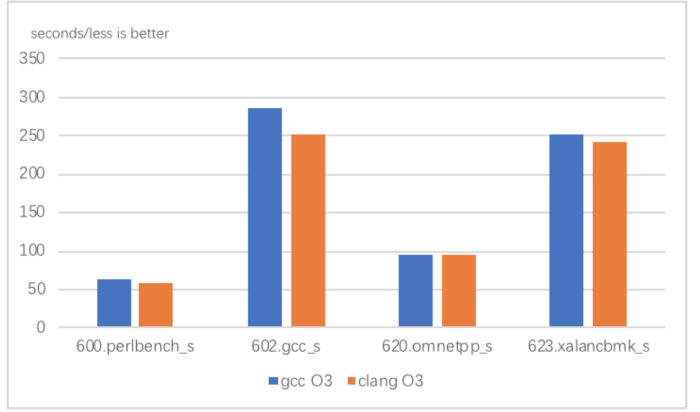
\includegraphics[scale=0.4]{CompilatoriGrafici/timeComparison.png}
 \caption{Tempo di compilazione}
 \label{Fig:Tempo di compilazione}
\end{figure}

Il processo di compilazione di GCC è il seguente: leggere il file sorgente, preelaborare il file sorgente, viene convertito in un IR, ottimizzato e generato un file assembly. Quindi l'assemblatore genera un file oggetto. 
Clang e LLVM non si basano su compilatori indipendenti, ma integrano compilatori auto-implementati nel back-end.  Rispetto a GCC, la struttura dei dati di LLVM, è più concisa e occupa meno memoria durante la compilazione ed è più veloce.  Pertanto, Clang  è vantaggioso in termini di tempo di compilazione, come dimostrano i dati ottenuti dalla compilazione \ref{Fig:Tempo di compilazione}.

\begin{figure}[h]
\centering
 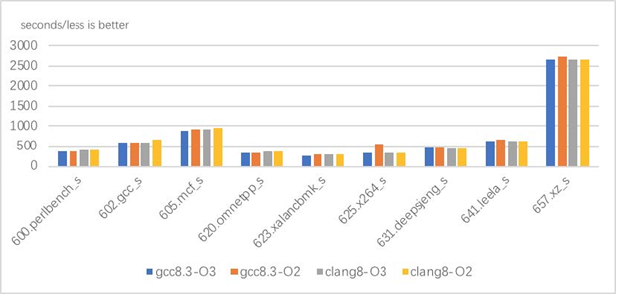
\includegraphics[scale=0.4]{CompilatoriGrafici/exeComparison.png}
 \caption{Performance di esecuzione}
 \label{Fig:Performance di esecuzione}
\end{figure}
Per valutare la performance i programmi sono stati compilati con l'opzione di ottimizzazione 2 e 3.

\subsection{Vantaggi dei compilatori}
\textbf{Compilatore GCC}
\begin{itemize}
	\item GCC supporta linguaggi più tradizionali rispetto a Clang e LLVM.
	\item GCC supporta architetture più meno popolari e supporta RISC-V prima di Clang e LLVM.
	\item GCC supporta più estensioni del linguaggio e più funzionalità del linguaggio assembly rispetto a Clang e LLVM.
\end{itemize}
\textbf{Compilatore CLANG}
\begin{itemize}
	\item I linguaggi emergenti utilizzano i framework LLVM, come Swift, Rust, Julia e Ruby.
	\item Clang e LLVM rispettano gli standard C e C++ in modo più rigoroso rispetto a GCC.
	\item Clang supporta anche alcune estensioni, come gli attributi per il controllo di sicurezza dei thread.
	\item Clang fornisce ulteriori utili strumenti, come scan-build e clang static Analyzer e altri per l'analisi statica, clang-format e clang-tidy per l'analisi della sintassi, nonché il plug-in dell'editor Clangd.
	\item Clang fornisce informazioni diagnostiche più accurate e intuitive ed evidenzia i messaggi di errore, le righe di errore, i prompt delle righe di errore e i suggerimenti per la riparazione. 
	\item Clang considera le informazioni diagnostiche come una caratteristica.
\end{itemize}

\subsection{Community}
E bene tener presente che entrambi i compilatori hanno delle community di supporto e di sviluppo per entrambi i progetti. 

\subsubsection{GCC Community}
Come altre comunità di software open source, la comunità GCC è dominata da appassionati di software libero. Nel processo di sviluppo, oggi si sono formanti dei meccanismi di gestione e partecipazione della comunità. Attualmente, la comunità GCC è una società relativamente stabile e ben definita in cui ogni persona ha ruoli e doveri chiari:

\begin{itemize}
\item Richard Stallman e Free Software Foundation (FSF): anche se raramente coinvolti nella gestione della comunità GCC, Richard Stallman e FSF sono ancora distaccati nelle licenze e negli affari legali.
\item Comitato industriale GCC: gestisce gli affari della comunità GCC, gli argomenti di sviluppo GCC indipendenti dalla tecnologia e la nomina e l'annuncio di revisori e manutentori. Attualmente conta 13 membri.
\item Manutentori globali: dominano le attività di sviluppo di GCC. In una certa misura, determinano il trend di sviluppo di GCC. Attualmente, ci sono 13 manutentori globali, che non ricoprono tutti cariche nel Comitato Industriale GCC.
\item Manutentori di frontend, middle-end e back-end: Sono responsabili del codice dei moduli di GCC corrispondente e molti di loro sono i principali contributori al codice del modulo. Vale la pena notare che i revisori sono generalmente classificati in questo gruppo. La differenza è che i revisori non possono approvare la propria patch, mentre i manutentori possono inviare le proprie modifiche nell'ambito della propria responsabilità senza l'approvazione dei revisori.
\item Collaboratori: sono i gruppi di sviluppatori più estesi nella comunità di GCC. Dopo aver firmato l'accordo sul copyright, tutti gli sviluppatori possono richiedere l'autorizzazione Scrivi dopo l'approvazione dalla community e quindi inviare il codice da soli.
\end{itemize}


Come altre comunità open source fanno gola alle società commerciali che hanno iniziato a svolgere ruoli importanti nella comunità, come il reclutamento di sviluppatori e la sponsorizzazione di riunioni di sviluppo. Attualmente, la comunità GCC è dominata dai seguenti tipi di società commerciali:
\begin{itemize}
\item Venditori di sistemi inclusi (RedHat, SUSE).
\item Venditori di chip (Intel, ARM, AMD, IBM).
\item Venditori specifici per determinati linguaggi o determinati servizi.
\end{itemize}

Nell'attuale comunità GCC, i fornitori di chip dominano lo sviluppo del back-end, mentre i fornitori di sistemi guidano altre aree di sviluppo. In termini di sviluppo della comunità, il codice GCC è attualmente ospitato sul proprio server SVN. Viene fornita un'API Git per facilitare lo sviluppo e l'invio. La revisione delle patch è simile a quella della comunità del kernel Linux e utilizza il modulo Mailing List. Come accennato in precedenza, la comunità GCC è una società di conoscenza relativamente stabile (o chiusa). La comunità ha fondamentalmente da 150 a 200 contributori attivi ogni anno e tiene una conferenza degli sviluppatori a settembre ogni anno. 

\subsubsection{LLVM Community}
La comunità LLVM è una comunità di compilatori giovane. Risponde rapidamente alle domande dei nuovi utenti e alle recensioni delle patch. 
Tutti i progetti e i problemi LLVM vengono discussi tramite l'elenco e-mail DevExpress e l'invio del codice viene notificato tramite l'elenco e-mail dei commit. Tutti i bug e le modifiche alle funzionalità vengono tracciati tramite l'elenco dei bug. Le patch inviate sono consigliate per i branch master. Lo stile è conforme agli standard di codifica LLVM e la revisione del codice viene eseguita tramite Phabricator. Attualmente, il repository di codice LLVM è stato migrato su GitHub.
A differenza della comunità GCC, la comunità LLVM ha solo la LLVM Foundation. La Fondazione LLVM ha otto membri. Oltre a gestire gli affari della comunità LLVM, ogni membro della LLVM Foundation deve guidare i problemi di sviluppo di LLVM relativi alla tecnologia. Attualmente il presidente è Tanya Lattner, moglie di Chris Lattner. Lo stesso Chris Lattner è anche un membro della fondazione e ha un forte controllo sulla comunità LLVM e sulla direzione dello sviluppo di LLVM.
La politica di revisione del codice nella comunità LLVM è sostanzialmente la stessa della comunità GCC. La differenza è che, a causa del rapido sviluppo di LLVM, molti contributori non hanno il permesso di accesso al commit e devono inviare il loro codice tramite i manutentori. Attualmente, le comunità Clang e LLVM hanno più di 1.000 contributori ogni anno. 


\section{Toolchain di RISC-V}
Per in alcuni sistemi non è presente nessun compilatore, per questi è possibile utilizzare la tecnica della cross-compilation (Sezione \ref{Sec:Cross}).  Per una cross-compilazione di base è necessario avere una toolchain. Una toolchain è l'insieme dei programmi usati nello sviluppo di un prodotto, tipicamente un altro programma o sistema di programmi. Tali strumenti sono utilizzati in catena in modo tale che producano del codice per un determinato dispositivo.\\
Per dispositivi RISC-V viene utilizzata la toolchain disponibile per LLVM/CLANG e GCC. Entrambe le toolchain sono mantenute dalle community, quella piu aggiornata e utilizzata è quella del progetto GNU.La documentazione e i vari tool sono disponibili sul loro \href{ http://riscv.org/software-tools/}{sito}.

\subsubsection{GCC toolchain}
La toolchain GNU RISC-V è composta da Binutils, newlib e glibc. La toolchain GCC si basa su GCC 6.1.0 e riceve commit su molto di frequente.  E' possibile usare uno script per creare l'intera toolchain per RISC-V. 
La toolchain di test utilizzata è stata RISC-V a 64bit.

\subsubsection{CLANG toolchain}
La toolchain di LLVM per RISC-V è iniziata nella versione LLVM 3.3 ed è attualmente stabile. Tuttavia, la versione 3.3 è piuttosto vecchia c'è anche un altra versione LLVM 3.8 meno stabile. La toolchain di di CLANG è piu macchinosa utilizzarla ma piu configurabile.  

\subsubsection{Comparazione}

Per la comparazione sono stati utilizzati RISC-V 32, 64 con i compilatori GCC e CLANG v 3.8. Il test eseguito è sulla dimensione del codice generato dai due compilatori. I programmi utilizzati fanno parte del benchmark MiBench.\footnote{a free, commercially representative embedded benchmark suite}.

\begin{figure}[h!]
	\centering
	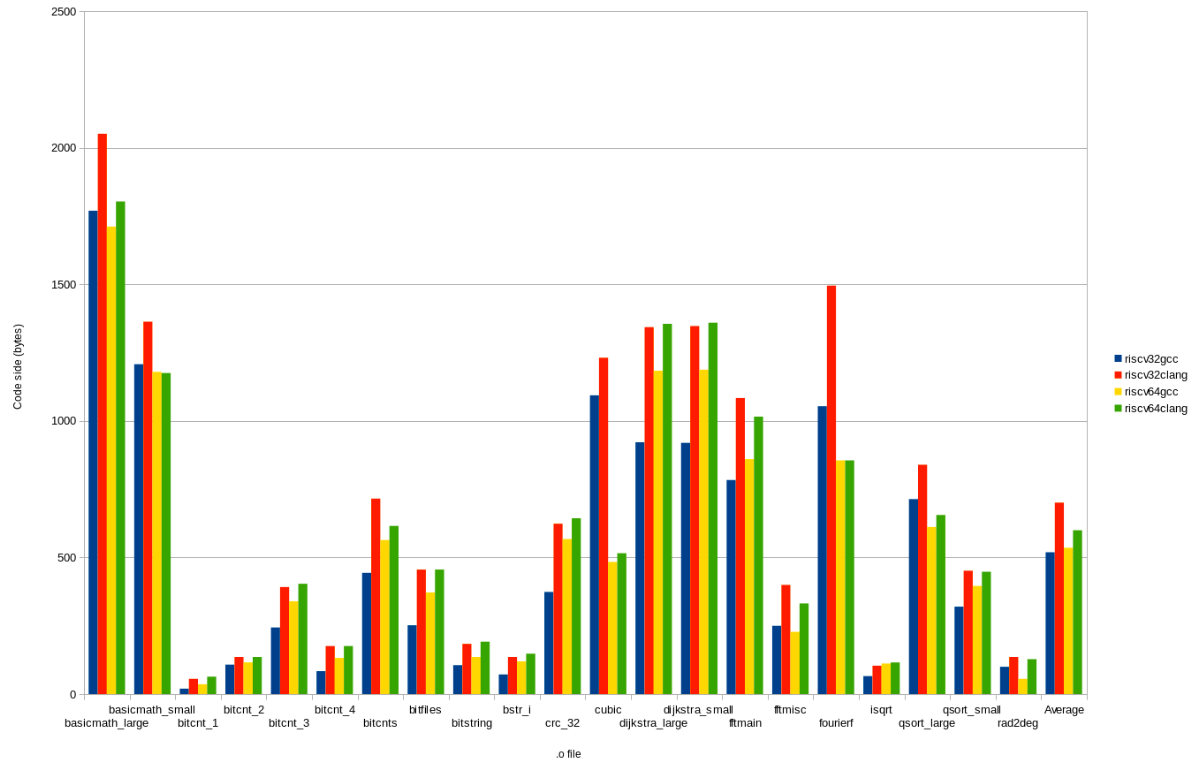
\includegraphics[scale = 0.3]{CompilatoriGrafici/Compilatori_GCC_CLANG.png}
	\caption{Confronto dimensione dei file generati dai compilatori}
	\label{Fig:graficoSizeComparisionCompilatori}
\end{figure}

\begin{table}[h!]
	\centering
	\begin{tabular}{| l | l | l |}
	\hline
		Compilatore & RISC-V 32 & RISC-V 64  \\ \hline
 	GCC	 & 519 bytes & 	536 bytes   \\ \hline
 	CLANG	 & 701 bytes &	600 bytes  \\ \hline
	\end{tabular}
	\caption{Dimensione media dei compilatori}
	\label{Tab:tabellaDimensioneMediaCompilatore}
\end{table}

In media, GCC produce dimensioni del codice abbastanza simili sia per RISC-V 32 che per 64. Il codice generato da Clang è leggermente più grande, in particolare per RISC-V 32, la cui dimensione del codice è in realtà maggiore rispetto a RISC-V 64. Questo puo dimostrare che CLANG puo essere ulteriormente migliorato. \\



\textbf{Comparazione del codice RISC-V e ARM}\\

\begin{figure}[h!]
	\centering
	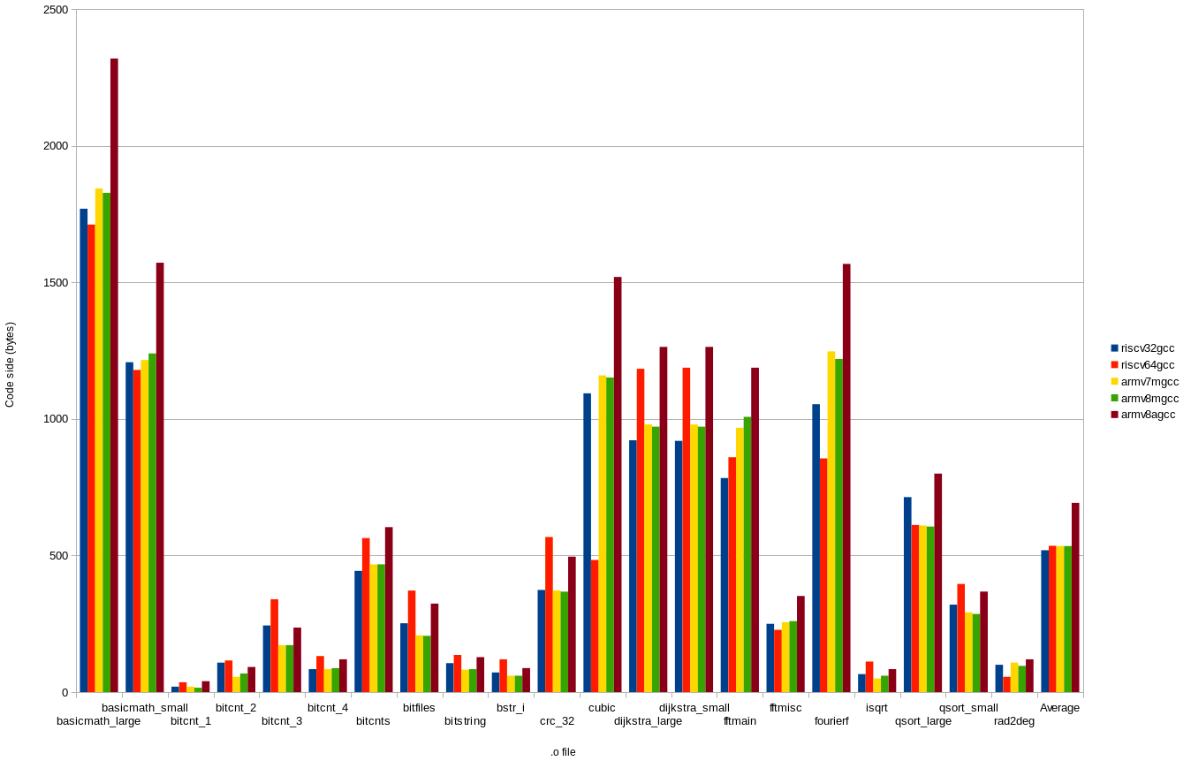
\includegraphics[scale = 0.3]{CompilatoriGrafici/SizeComparision_ARM_RISCV.png}
	\caption{Confronto dimensione}
	\label{Fig:graficoSizeComparision}
\end{figure}

\begin{table}[h!]
	\centering
	\begin{tabular}{| l | l |}
	\hline
	Architettura & Dimensione media \\ \hline
	RISC-V 32	 & 519 bytes  \\ \hline
 	RISC-V 64	 & 536 bytes  \\ \hline
 	ARMv7m	 & 535 bytes  \\ \hline
 	ARMv8m	 & 535 bytes  \\ \hline
 	ARMv8a	 & 693 bytes  \\ \hline
	\end{tabular}
	\caption{Dimensione media}
	\label{Tab:tabellaDimensioneMediaArch}
\end{table}

\newpage
\textbf{Confronto tra le architetture}\\
In Conclusione le toolchain si comporta come aspettato. Il compilatore GCC produce codice piu contenuto della controporte CLANG, le rispettive toolchain si comportano allo stesso modo.
Al momento, la toolchain GCC per RISC-V produce codice che è in media il 18\% più piccolo del codice prodotto dalla toolchain LLVM per un sottoinsieme dei benchmark MiBench. Per lo stesso insieme di benchmark, il codice RISC-V 64 ha le stesse dimensioni del codice ARMv7m e ARMv8m. Il codice RISC-V 32 è circa il 3\% più piccolo del codice RISC-V 64, ARMv7m e ARMv8m.



\chapter{BenchMarking}
\todo{Rileggi/Correggi capitolo 4: Benchmarking}
\section{Descrizione board}

La scheda di sviluppo utilizzata è  D1-H Nezha basata sul design del chip Allwinner D1-H. La board integra una CPU Ali Pingtou Ge RISC-V C906, con clock a 1 GHz, supporta il kernel Linux standard, supporta  2G DDR3, 258 MB di spin-nand, WiFi/Bluetooth connessione, con interfacce audio e video,  può essere collegato a varie periferiche, interfaccia MIPI-DSI+TP integrata, interfaccia scheda SD,interfaccia HDMI, interfaccia scheda figlia microfono, interfaccia auricolari da 3,5 mm , interfaccia Gigabit Ethernet, USB HOST, interfaccia di tipo C, interfaccia di debug UART, array di pin a 40 pin.

\begin{figure}[h!]
\includegraphics[width = \textwidth]{D1H-BoardTopView.png}
\caption{Board vista dall' alto}

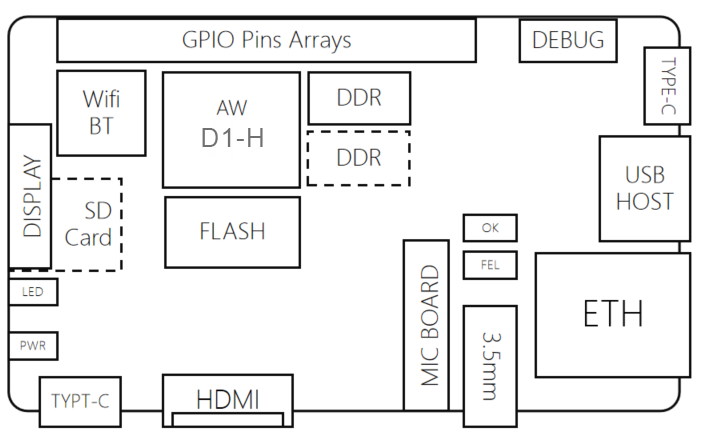
\includegraphics[width = \textwidth]{D1H-BoardBlockView.png}
\caption{Schema a blocchi della scheda di sviluppo}
\end{figure}

\vspace{2cm}
\begin{table}[h!]
\centering
\begin{tabular}{|r|c|}
\hline
CPU & Allwinner D1-H \\
\hline
Clock & 1GHz\\
\hline
DRAM & DDR3 2GB\\
\hline
Memoria & 256MB  spin-nand integrato\\
\hline 
Supporto memoria & USB e  SD\\
\hline
Rete & Gigabit Ethernet,  2.4G WiFi e Bluetooth , antenna integrata\\
\hline
Display & MIPI-DSI + TP, HDMI, SPI \\
\hline
Audio & jack per cuffie da 3,5 mm\\
\hline
Tasti & FEL, LRADC OK\\
\hline
Luci &  alimentazione, LED tricolore\\
\hline
DEBUG & UART, USB ADB\\
\hline
USB & USB , USB OTG, USB2.0\\
\hline
PIN & array di pin 40\\
\hline
Alimentazione & USB-C  5V-2A\\
\hline
Dimensioni & lunghezza 85 mm * larghezza 56 mm * spessore 1,7 mm\\
\hline

\end{tabular}
\caption{Caratteristiche della board}
\end{table}

\section{Ambiente di sviluppo}
La scheda di sviluppo D1-H viene fornita con il sistema Tina Linux. Il kernel fornito  adattato al kernel Linux 5.4. La board fornisce il supporto di base e gestione delle risorse hardware del dispositivo. Ulteriori informazioni sono disponibili sul sito della \href{https://d1.docs.aw-ol.com/study/study_1tina/}{board}.

\section{Presentazione programmi}
I programmi utilizzati sono scritti in C e sono contenuti su github su una \href{https://github.com/MattiaBianchessi/Testing_RISC-V}{repository}.
 Ogni directory contiene i dati di esecuzione di ciascun programma eseguito sulla board in un file con estensione .csv e un notebook jupyter per visualizzare i dati e, in alcuni casi confrontarli.
\subsection{Operazioni Aritmetiche}
Operazioni: la directory contiene un programma che esegue le operazioni aritmetiche di base 
\begin{itemize}
	\item addizione
	\item sottrazione
	\item moltiplicazione
	\item divisione
	\item modulo
\end{itemize} 
Il programma genera due matrici quadrate di numeri interi su cui vengono eseguite le operazioni elemento per elemento. Le dimensioni delle matrici sono 1000 x 1000, 2500 x 2500, 5000 x 5000, 8000 x 8000, 10000 x 10000, 15000 x 15000.

La prima matrice generata ha valori tra 1 e 200, la seconda ha valori tra 1 e 100.

Per ogni matrice vengono eseguite 5 prove da cui viene calcolato il tempo medio di esecuzione

\subsection{Prime Number}
Il programma generai primi 5000 numeri primi. Viene calcolato il tempo di esecuzione. Nella directory sono presenti 2 programmi. Il primo 'prime.c' che controlla da 2 in poi se n-esimo numero è divisibile. 
\todo{Analizza costo algoritmo}
Il secondo utilizza il crivello di Atkin per calcolare i numeri primi. \todo{Info Sieve of Atkin}.

\subsection{Moltiplicazione o shift}
Il programma confronta la velocità di esecuzione di moltiplicazione e divisione aritmetiche con lo shift. Il programma genera un array di interi di valori tra 0 e maxInt e un array di potenze di 2 comprese tra 2 e 1024. Entrambi gli array hanno 1000 elementi. Dopo la generazione viene calcolato elemento per elemento il risultato e viene memorizzato il tempo di esecuzione. Il risultato del programma è il tempo medio di esecuzione di 1000 operazioni per tipo (moltiplicazione normale, divisione normale, moltiplicazione tramite shift, divisione tramite shift).

\subsection{Montecarlo Pi}
Algoritmo di approssimazione del pigreco tramite il metodo di montecarlo. Nell esecuzione vengono utilizzati da 10 a ($ 10^{10} $) punti per l'approssimazione. Ogni iterazione viene eseguita 5 volte e per ogni iterazione viene memorizzato il valore calcolato con il proprio tempo di esecuzione. Il programma si basa sulla funzione rand.

\subsection{Sorting}
Gli algoritmi di sorting utilizzati sono:
\begin{itemize}
	\item BubbleSort
	\item InsertionSort
	\item QuickSort
	\item HeapSort
\end{itemize}

Ogni algoritmo viene eseguito su array di dimensione diversa 500, 1000, 5000, 10000, 20000, 35000, 50000. Per ogni set vengono eseguite 150 prove sulle quali viene calcolato il tempo di esecuzione. Il programma informa per ogni gruppo di array il tempo massimo, il minimo e il tempo medio. Per alcuni algoritmi vengono utilizzate anche delle configurazioni particolari dell array da ordinare, come ad esempio utilizzando il BubbleSort vengono oridinati array strettamente crescenti e strettamente decrescenti oltre che ai campioni casuali. Nella situazione generale gli array vengono generati con numeri interi casuali.
\todo{Info arlogitmi}

\subsection{BackTracking}

In questa direcotry sono contenuti due programmi:

Un solutore di sudoku
Un solutore di labirinti
In entrambi i casi vengono utilizzate tecniche di backtracking. Lo scopo è quello di valutare il tempo di esecuizione di programmi che fanno uso del backtracking su processore RISC.

Sudoku
Nel file sudoku.h sono presenti 8 sudoku di varia difficoltà, 2 di essi non sono fattibili, uno per costruzione(sbagliato in partenza) e l 'altro è impossibile risolverlo per la configurazione.

MazeSolver
Questa directory è presente il file mazeGen.py che è stato utilizzato come generatore di labirinti. Il solutore mazeSolver.c, una volta in esecuzione, chiede il path del labirinto da risolvere e successivamente è possibile salvare la soluzione, se trovta, in un nuovo file.

Labirinto personale
Il file con estensione .txt, se si vuole utilizzare un altro labirinto, dovrà avere:

sulla prima linea il numero di linee del labirinto.
sulla seconda linea il numero di colonne.
dalla terza in poi il labirinto che dovrà avere un simbolo , come ad esempio '\#', per indicare i muri, lo spazio ' ' per indicare i corridoi, uno e un solo simbolo 'I' per indicare l' inizio e uno e un solo simbolo 'O' per indicare l' uscita del labirinto.
Sono presenti alcuni esempi nella sottodirectory maze di labirinti.


\chapter{Comparativa}

\section{Operazioni}
	Con il programma operazioni viene visualizzato il tempo di esecuzione di alcune operazioni matematiche di base. Come mostrato nelle porzioni di codice Code \ref{Code:Sum},\ref{Code:Sub}, \ref{Code:Mul}, \ref{Code:Div}, \ref{Code:Mod} mostrano le funzioni che si occupano delle operazioni. Ogni funzione, semplicemente, cicla ogni elemento dell' array a e dell array b, ne esegue l'operazione e memorizza il risultato in un array c. L'array a ha valori interi compresi tra 1 e 200, l'array b ha valori interi compresi tra 1 e 100,  le matrici utilizzate sono matrici quadrate e le dimensioni utilizzate sono 1000, 2500, 5000, 8000, 10000, 15000. Per ogni operazione vengono eseguite 5 prove da cui viene calcolato il tempo medio di esecuzione. 
	Per riferimento il programma è stato utilizzato anche su un MacBook Air. 
	
	\lstinputlisting[language=c,  style = Cstyle, caption = Addizione,  label ={Code:Sum} ]{PorzioniCodice/Operazioni/sum.c}
	\lstinputlisting[language=c,  style = Cstyle, caption = Sottrazione, label ={Code:Sub}]{PorzioniCodice/Operazioni/sub.c}
	\lstinputlisting[language=c,  style = Cstyle, caption = Moltiplicazione, label ={Code:Mul}]{PorzioniCodice/Operazioni/mul.c}
	\lstinputlisting[language=c,  style = Cstyle, caption = Divisione, label ={Code:Div}]{PorzioniCodice/Operazioni/div.c}
	\lstinputlisting[language=c,  style = Cstyle, caption = Modulo, label ={Code:Mod}]{PorzioniCodice/Operazioni/mod.c}
	
	Di seguito vengono riportati i tempi di esecuzione medi per operazione e per dimensione
	\begin{table}[h!]
	
	\centering
	\begin{tabular}{| l | c | c | c | c | c | c |}
		\hline
		Operazione & 1000 & 2500 & 5000 & 8000 & 10000 & 15000 \\ \hline
		Somma & 0.002317 & 0.013848 & 0.055129 & 0.142010 & 0.227784 & 0.504650\\ \hline
		Sottrazione & 0.002324 & 0.013921 & 0.054900 & 0.142941 & 0.227505 & 0.504767\\ \hline
		Prodotto & 0.002344 & 0.014010 & 0.055036 & 0.143293 & 0.226141 & 0.504829\\ \hline
		Divisione & 0.002352 & 0.013953 & 0.055298 & 0.142226 & 0.227948 & 0.505007\\ \hline
		Modulo & 0.002298 & 0.013880 & 0.055009 & 0.142129 & 0.227835 & 0.505035\\ \hline

	\end{tabular}
	
	\caption{Tempi di esecuzione MacBook-Air}
	\end{table}
	
	\begin{table}[h!]
		\centering
		\begin{tabular}{{| l | c | c | c | c | c | c |}}
			\hline
			Operazione & 1000 & 2500 & 5000 & 8000 & 10000 & 15000   \\ \hline	
			Somma & 0.011256 & 0.069917 & 0.279804 & 0.714786 & 1.117411 & 2.512942  \\ \hline	
			Sottrazione & 0.011237 & 0.069850 & 0.279895 & 0.714680 & 1.117352 & 2.512978  \\ \hline	
			Prodotto & 0.011234 & 0.069899 & 0.279219 & 0.715381 & 1.117296 & 2.514183  \\ \hline	
			Divisione & 0.011170 & 0.069781 & 0.279884 & 0.714673 & 1.116763 & 2.513539  \\ \hline	
			Modulo & 0.011212 & 0.069845 & 0.279913 & 0.715371 & 1.117348 & 2.514198  \\ \hline	
		\end{tabular}
		
	\caption{Tempi di esecuzione RISC-V}
	\end{table}
	Di seguito i grafici rappresentativi delle tabelle precedenti.
	\begin{figure}
	\centering
		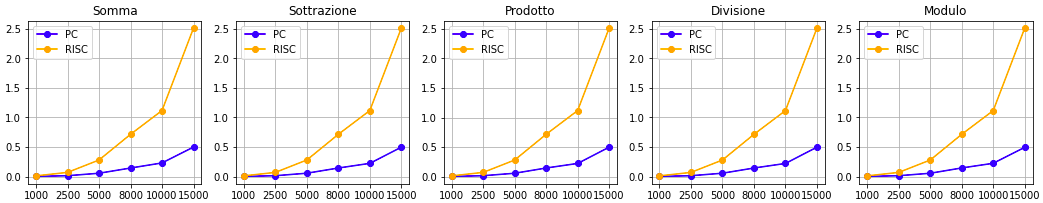
\includegraphics[scale= 0.4]{PorzioniCodice/Operazioni/Grafico.png}
	\end{figure}
	Prendiamo in considerazione l'operazione di somma del processore RISC. Il tempo di esecuzione per la matrice 1000 x 1000 è di 0.011256 e per la matrice 2500 x 2500 è di  0.069917 il che è 6.2115 (circa) il tempo di esecuzione e 6.25 la dimensione dei dati.  Per il MacBook il tempo di esecuzione per la matrice 1000 x 1000 è di 0.002317 e per la matrice 2500 x 2500 è di  0.013848 il che è 5.97 (circa) il tempo di esecuzione e 6.25 la dimensione dei dati.  i tempi di esecuzioni della stessa operazione sono piu o meno lo stesso valore e il rapporto rimane simile per tutte le operazioni.
	Il tempo di esecuzione totale del programma è di 23.653595 per Macbook mentre 117.665045 per RISC. Quindi il MacBook è 4.97 \% piu veloce del processore RISC, risultato abbastanza prevedibile. Confrontando le architetture il processore del MacBook è di 2.2 GHz con memoria da 8Gb da 1600MHz mentre il processore RISC è di 1 GHz con memoria da 2Gb a 1333 MHz.
	Avere una CPU da 1 Hertz significa avere un processore che può fare una cosa al secondo,  quindi il processore del Mac può eseguire 2.2 miliardi di operazioni in un solo secondo di contro il processore RISC solamente 1 miliardo, meno della metà invece la memoria RAM il processore RISC è di 2Gb con 1333 MHz di frequenza e il MacBook 8Gb con 1600 MHz.



\section{PrimeNumber}
Il programma utilizza una scansione lineare per trovare i primi 5000 numeri primi. In seguito viene mostrato il codice della funzione principale.  La funzione controlla dal numero 2 in avanti se il numero è primo, se lo è viene inserito nell array altrimenti no e il ciclo viene eseguito fino a trovare 5000 numeri primi.  

\lstinputlisting[language=c,  style = Cstyle, caption = Impostazioni dei dati,  label ={Code:prime} ]{PorzioniCodice/Prime/prime.c}

I file sono stati compilato con diverse livelli di ottimizzazione.
\begin{table}[h]
\begin{tabular}{|l|c|r|}
\hline
    & PC       & RISC-V    \\ \hline
-O2 & 0.041286 & 0.434372  \\ \hline
-O1 & 0.033024 & 0.346976  \\ \hline
-O0 & 0.032363 & 0.3122784 \\ \hline
\end{tabular}
\caption{Tempi di esecuzione numeri primi}
\label{Tab:TempoPrime}
\end{table}
Come precedentemente notato è l'ordine di grandezza di differenza dei due processori. Andando a guardare nei sorgenti assembly notiamo delle differenze. La prima abbastanza ovvia è la dimensione del file che nel caso dell ottimizzazione 0 è superiore (172 linee 4KB) rispetto all livello 2 (130 linee 4KB).Il secondo è l'utilizzao dell'istruzione nop nell livello 0.
Il codice \ref{Code:primeO0} fa riferimento alla porzione di codice dove vengono utilizzate le istruzioni nop.\\

\lstinputlisting[language = Risc-v,  caption =Sorgente prime ottimizzato con -O0,  label ={Code:primeO0},  firstline=48,lastline=55 ]{PorzioniCodice/Prime/prime0.s}

La pseudo-istruzione nop(No operation) ha come implementazione addi x0, x0, 0 è intiutivo capre che somma zero (costante) al registro contenente zero (x0) e lo memorizza nel registro x0. Questo è un caso eccezionale in cui si ha la possibilità di scrivere il registro x0, seppur con poco significato algebricamente, ogni altro caso in cui si vuole modificare il registro x0 solleverebbe errori. La motivazione della presenza di queste operazioni è più un fatto storico.
La maggior parte delle implementazioni hardware ha degli interlock. Se un'istruzione necessita di dati che non sono ancora disponibili, la pipeline si interrompe finché i dati non sono disponibili. Oppure, se si tratta di una pipeline di esecuzione fuori ordine, un'istruzione si blocca finché i dati non sono disponibili e altre istruzioni possono continuare l'esecuzione.\\
I nop emessi dal compilatore con -O0  non vengono emessi a -O1 o superiore. Un ulteriore modo di utilizzo dell istruzione nop è quello di confronto diretto tra i sorgenti compilati con livelli di ottimizzazione differente. Il compilatore emette delle operazioni nop  in modo da avere un posto dove allegare le informazioni sul numero di riga con il comando -g durante la compilazione. Se una destinazione non dispone di interblocchi hardware, è compito del backend di destinazione aggiungere eventuali nop che potrebbero essere necessari per il corretto funzionamento sulla destinazione. Al momento non ci sono target RISC-V supportati da gcc che lo richieda.



\section{MultOrShift}
Il programma confronta la velocità di esecuzione di moltiplicazione e divisione aritmetiche con lo shift. Il programma genera un array di interi di valori tra 0 e maxInt e un array di potenze di 2 comprese tra 2 e 1024. Entrambi gli array hanno 1000 elementi. Dopo la generazione viene calcolato elemento per elemento il risultato e viene memorizzato il tempo di esecuzione. Il risultato del programma è il tempo medio di esecuzione di 1000 operazioni per tipo (moltiplicazione normale, divisione normale, moltiplicazione tramite shift, divisione tramite shift). Di seguito alcune porzioni di codice:

\lstinputlisting[language=c,  style = Cstyle, caption = Impostazioni dei dati,  label ={Code:Init} ]{PorzioniCodice/MultShift/init.c}
\lstinputlisting[language=c,  style = Cstyle, caption = Impostazioni dei dati,  label ={Code:Mult} ]{PorzioniCodice/MultShift/Mult.c}
\lstinputlisting[language=c,  style = Cstyle, caption = Impostazioni dei dati,  label ={Code:Shift} ]{PorzioniCodice/MultShift/Shift.c}

Il codice \ref{Code:Init} imposta i due array.  I codici \ref{Code:Mult} e \ref{Code:Shift} mostrano l'operazione eseguita.
La tabella \ref{Tab:tempi_esecuzioneMS} mostra i tempi di esecuzione calcolati in millisecondi delle varie operazioni.

\begin{table}[h]
\centering
\begin{tabular}{lcccc}
\cline{2-5}
\multicolumn{1}{l|}{}         & \multicolumn{2}{c|}{PC}                                   & \multicolumn{2}{c|}{RISC-V}                               \\ \hline
\multicolumn{1}{|l|}{Normale} & \multicolumn{1}{c|}{0.0036} & \multicolumn{1}{c|}{0.0042} & \multicolumn{1}{c|}{0.0430} & \multicolumn{1}{c|}{0.0572} \\ \hline
\multicolumn{1}{|l|}{Shift}   & \multicolumn{1}{c|}{0.0034} & \multicolumn{1}{c|}{0.0034} & \multicolumn{1}{c|}{0.0404} & \multicolumn{1}{c|}{0.0826} \\ \hline
                              & \multicolumn{1}{l}{}        & \multicolumn{1}{l}{}        & \multicolumn{1}{l}{}        & \multicolumn{1}{l}{}       
\end{tabular}
	\label{Tab:tempi_esecuzioneMS}
	\caption{Tempi di esecuzione operazioni calcolati in ms}
\end{table}
	
	
\section{analisi codice assembly}
Osserviamo i compilatori a confronto.  I Compilatori confrontati sono \textit{gcc RISC-V},  \textit{gcc ARM} e \textit{gcc x86\_64}.  I compilatori RISC-V e ARM vengono confrontati per il loro focus sul ambiente embedded ed entrambi sono architetture RISC.Tutti i codici presentati in questa sezione vengono compilati e presentati con il livello di ottimizzazione di default (-O0).


\section{Operazioni}
\subsection{Addizione con costante}

\lstinputlisting[language=c,  style = Cstyle,  caption = Addizione, label = {Code:AddComp}]{PorzioniCodice/ConfrontoCompilatori/C/get_num.c}

La funzione è una semplice funzione scritta in C che dato un numero di tipo intero restituisce il numero sommato a 23. 

\vspace{0.3 cm}
\textbf{RISC-V}

\vspace{0.3 cm}
Il sorgente compilato con il compilatore RISC-V \ref{Code:AddRISCV} da riga 2 fino a riga 6 predispone la chiamata della procedura posizionando sullo stack il necessario, da riga 7 inizia la funzione. Su quella riga viene recuperato il valore di num che alla riga 8, tramite l'operazione di add immediate, viene sommato a num. Il risultato dell operazione addiw è la somma del valore di num sommato alla costante 23, il risultato è esteso su 64 bit, vengono ignorati gli errori di overflow. Successivamente tramite la pseudo istruzione sext.w che prende i 32 bit inferiori e li memorizza nel registro rd.  Questa istruzione corrisponde a addiw rd, rs,1 0. Il risultato viene spostato nel registro a0 che, nei processori RISC-V, viene utilizzato come restituzione di risultato. Le righe successive ripristinano lo stack e restituice il controllo al chiamante.

\vspace{0.3 cm}
\textbf{ARM}

\vspace{0.3 cm}

l sorgente  \ref{Code:Addx86} , compilato con gcc ARM, mostra che la preparazione della procedure si esegue da riga 2 a riga 5, le con le due righe successive si esegue la funzione. La riga 6 recupera il valore di num la riga successiva calcola il valore del risultato e, infine, alla riga 8 si sposta il risultato nel registro di restituzione


\vspace{0.3 cm}
\textbf{x86}

l sorgente  \ref{Code:AddARM} è compilato con gcc di x86.  Da riga 2 fino a riga 4 viene preparato lo stack, a riga 5 viene posizionato num nel registro eax che a riga 6 viene sommato a 23 che viene memorizzato nel registro eax. Infine viene ridato il controllo al chiamante.

\vspace{0.3 cm}

\begin{figure}[h!]
     
     \begin{subfigure}{0.3\textwidth}
  
        \lstinputlisting[language = Risc-v]{PorzioniCodice/ConfrontoCompilatori/Assembler/RISC-V/get_num.txt}
\label{Code:AddRISCV}
\caption{RISC-V}
     \end{subfigure}
     \hfill
     \begin{subfigure}{0.3\textwidth}
         
          \lstinputlisting[language = Risc-v]{PorzioniCodice/ConfrontoCompilatori/Assembler/ARM/get_num.txt}
\caption{ARM}
\label{Code:AddARM}
     \end{subfigure}
     \hfill
     \begin{subfigure}{0.3\textwidth}
         
          \lstinputlisting[language = Risc-v]{PorzioniCodice/ConfrontoCompilatori/Assembler/x86/get_num.txt}
	 \caption{x86}
	\label{Code:Addx86}
     \end{subfigure}
    
        \caption{Funzione di somma}
        
\end{figure}

\subsection{Addizione}
Nel caso generale viene calcolata la somma di 3 numeri.
\lstinputlisting[language=C,  style = Cstyle,  caption = {Addizione generale}, label = {Code:Add2Comp}]{PorzioniCodice/ConfrontoCompilatori/C/sumGen.c}


\vspace{0.3 cm}
\textbf{RISC-V}

Nel caso del compilatore RISC-V la somma avviene tra 13 e 19 dove gli operandi vengono caricati nei registri a4 e a5,  successivamente calcolato il risultato e memorizzato in a4 che poi verrà sommato con l'ultimo operando, caricato a riga 17.

\vspace{0.3 cm}
\textbf{ARM}

Nel caso ARM avviene lo stesso meccanismo. Tra le righe 8 e 12 avviene il caricamento dei primi due operandi la somma parziale e infine la somma totale.

\vspace{0.3 cm}
\textbf{x86}

Infine per x86 il calcolo avviene tra le righe 7 e 11 nello stesso modo con cui viene eseguito in ARM.

\begin{figure}[h]
     
     \begin{subfigure}[b]{0.3\textwidth}
  
        \lstinputlisting[language = Risc-v, caption = Addizione RISC-V] {PorzioniCodice/ConfrontoCompilatori/Assembler/RISC-V/sumGen.txt}
	\label{Code:Add2RISC}
\caption{RISC-V}
     \end{subfigure}
     \hfill
     \begin{subfigure}[b]{0.3\textwidth}
         
          \lstinputlisting[language = Risc-v]{PorzioniCodice/ConfrontoCompilatori/Assembler/ARM/sumGen.txt}
          \label{Code:Add2ARM}
\caption{ARM}
     \end{subfigure}
     \hfill
     \begin{subfigure}[b]{0.3\textwidth}
         
          \lstinputlisting[language = Risc-v]{PorzioniCodice/ConfrontoCompilatori/Assembler/x86/sumGen.txt}
	 \caption{x86}
	\label{Code:Add2X86}
     \end{subfigure}
    
        \caption{Funzione di somma}
        
\end{figure}



\subsection{Moltiplicazione}

\vspace{0.3 cm}
\textbf{Moltiplicazioni per potenze di 2}

\lstinputlisting[language=C,  style = Cstyle,  caption = {Moltiplicazione per potenza di 2}, label = {Code:Mul2Comp}]{PorzioniCodice/ConfrontoCompilatori/C/mult2.c}

La funzione dato un numero di tipo intero restituisce il numero moltiplicato per 2.  Per i sorgenti le parti di preparazione sono simili per le rispettive preparazioni precedenti.



\vspace{0.3 cm}
Nel sorgente RISC-V \ref{Code:Add2RISC} l'operazione di moltiplicazione per 2 avviene tramite uno shift logical left di 1 bit (SLLIW). Stesso concetto avviene nel sorgente ARM \ref{Code:Add2X86} dove l 'operazione di moltiplicazione per 2 avviene tramite lo shift left di 1 bit. Invece nel sorgente x86 \ref{Code:Add2ARM} la moltiplicazione avviene tramite una somma. Questa somma è un caso particolare, infatti se volessimo moltiplicare per una qualsiasi potenza di 2 (ad esempio in figura 3) le operazioni avvengono tutte tramite shift left di un opportuno valore. Con la figura 4 viene mostrato il calcolo di una moltiplicazione per 8. Nei casi RISC-V e ARM il calcolo avviene attraverso Shift e nel caso x86 avviene anche qui uno shift.


\vspace{0.3 cm}

\begin{figure}
     
     \begin{subfigure}[b]{0.3\textwidth}
  
        \lstinputlisting[language = risc-v]{PorzioniCodice/ConfrontoCompilatori/Assembler/RISC-V/mult2.txt}
        
	\caption{RISC-V}
	\label{Code:Mul2RISC}
     \end{subfigure}
     \hfill
     \begin{subfigure}[b]{0.3\textwidth}
         
          \lstinputlisting[language = risc-v]{PorzioniCodice/ConfrontoCompilatori/Assembler/ARM/mult2.txt}	
		\caption{ARM}
		\label{Code:Mul2ARM}
     \end{subfigure}
     \hfill
     \begin{subfigure}[b]{0.3\textwidth}
         
          \lstinputlisting[language = risc-v]{PorzioniCodice/ConfrontoCompilatori/Assembler/x86/mult2.txt}
	 \caption{x86}
	\label{Code:Mul2X86}
     \end{subfigure}
     \caption{Moltiplicazione per 2}
     \end{figure}
 	
 \begin{figure}
     \begin{subfigure}[b]{0.3\textwidth}
         
          \lstinputlisting[language = risc-v]{PorzioniCodice/ConfrontoCompilatori/Assembler/RISC-V/mult8.txt}	
		\caption{RISC-V}
		\label{Code:Mul8RISC}
     \end{subfigure}
     \hfill
     \begin{subfigure}[b]{0.3\textwidth}
         
          \lstinputlisting[language = risc-v]{PorzioniCodice/ConfrontoCompilatori/Assembler/ARM/mult8.txt}	
		\caption{ARM}
		\label{Code:Mul8ARM}
     \end{subfigure}
     \hfill
     \begin{subfigure}[b]{0.3\textwidth}
         
          \lstinputlisting[language = risc-v]{PorzioniCodice/ConfrontoCompilatori/Assembler/x86/mult8.txt}	
		\caption{x86}
		\label{Code:Mul8X86}
     \end{subfigure}
    
        \caption{Moltiplicazione per 8}
        
\end{figure}

\vspace{0.3 cm}

\textbf{Moltiplicazione per una costante}

Vengono presentati due codici molto simili, il primo moltiplica il numero per 31 che rappresenta più in generale un numero che dista da una potenza di 2 di 1. Il secondo è un caso più generale dove avviene la moltiplicazione di un numero non potenza di due e che dista da una potenza almeno di 2, nel nostro caso il numero è 30.

\vspace{0.2 cm }

\begin{figure}[h]
	\begin{subfigure}[b]{0.4\textwidth}
         
          \lstinputlisting[language=C,  style = Cstyle, label = {Code:Mul31Comp}]{PorzioniCodice/ConfrontoCompilatori/C/mult31.c}	
		
     \end{subfigure}
     \hfill
     \begin{subfigure}[b]{0.4\textwidth}
         
          \lstinputlisting[language=C,  style = Cstyle, label = {Code:Mul30Comp}]{PorzioniCodice/ConfrontoCompilatori/C/mult30.c}	
		
     \end{subfigure}
     
\end{figure}

\vspace{0.3 cm}

Nel caso della moltiplicazione per 31 l'approccio dei 3 sorgenti è identico. Viene calcolata la moltiplicazione per 32 attraverso shift logici e poi viene sottratto una volta il valore per ottenere la moltiplicazione per 31. Se il valore costante fosse 33 , il numero successivo alla potenza di 2, l' operazione di sottrazione viene sostituita con una di addizione. Nel caso più generale invece abbiamo un approccio differente.\\
Partendo dall x86 la moltiplicazione avviene semplicemente con l'istruzione imul a riga 6.  Nel caso ARM l'operazione di moltiplicazione viene comunque eseguita da una singola istruzione(riga 8) ma vengono utilizzati i registri r2 e r3 che precedentemente (riga 6 e 7) vengono riempiti con gli operandi. Infine l' implementazione di RISC-V utilizza ancora shift. Nel caso della moltiplicazione per 30 avviene prima uno shift di 4 ( moltiplicazione per 16) successivamente sottratto una volta il numero e infine al risultato avviene applicato uno shift di 1 (moltiplicazione per 2). \\ Quindi: \\ 
$((num * 2^4) - num ) * 2^1 = $ 

$ =((num * 16 ) - num ) * 2 =$ 

$ = 15 * num * 2 =  num *30 $ 

\vspace{0.2 cm}
In generale RISC-V utilizza opportuni shift combinate con addizioni e sottrazioni per ottenere il valore della costante.

\begin{figure}[h]

     \begin{subfigure}[b]{0.3\textwidth}
  
        \lstinputlisting[language = risc-v]{PorzioniCodice/ConfrontoCompilatori/Assembler/RISC-V/mult31.txt}
        \label{Code:Mul31RISC}
	\caption{RISC-V}

     \end{subfigure}
     \hfill
     \begin{subfigure}[b]{0.3\textwidth}
         
          \lstinputlisting[language = risc-v]{PorzioniCodice/ConfrontoCompilatori/Assembler/ARM/mult31.txt}	
		\caption{ARM}
		 \label{Code:Mul31ARM}
     \end{subfigure}
     \hfill
     \begin{subfigure}[b]{0.3\textwidth}
         
          \lstinputlisting[language = risc-v]{PorzioniCodice/ConfrontoCompilatori/Assembler/x86/mult31.txt}
	 \caption{x86}
	 \label{Code:Mul31X86}
     \end{subfigure}
     \caption{Moltiplicazione per 31}
     \end{figure}

\begin{figure}

     \begin{subfigure}[b]{0.3\textwidth}
  
        \lstinputlisting[language = risc-v]{PorzioniCodice/ConfrontoCompilatori/Assembler/RISC-V/mult30.txt}
         \label{Code:Mul30RISC}
	\caption{RISC-V}

     \end{subfigure}
     \hfill
     \begin{subfigure}[b]{0.3\textwidth}
         
          \lstinputlisting[language = risc-v]{PorzioniCodice/ConfrontoCompilatori/Assembler/ARM/mult30.txt}	
		\caption{ARM}
		 \label{Code:Mul30ARM}
     \end{subfigure}
     \hfill
     \begin{subfigure}[b]{0.3\textwidth}
         
          \lstinputlisting[language = risc-v]{PorzioniCodice/ConfrontoCompilatori/Assembler/x86/mult30.txt}
	 \caption{x86}
	 \label{Code:Mul30X86}
     \end{subfigure}
     \caption{Moltiplicazione per 30}
     \end{figure}

\vspace{2cm}

\subsection{Divisione}

Per quanto riguarda la divisione viene utilizzato la stessa metodologia della moltiplicazione.




\section{MonteCarloPi}
% valutazione generatore numeri casuali 
Al giorno d'oggi è comune utilizzare la generazione di numeri casuali in tecniche o simulazioni, ad esempio numeri di conto bancario e crittografia. È una tecnica necessaria e di base nella programmazione di computer. Non è possibile avere un generatore scelto tra tanti senza valutarne la casualità. Ad esempio un generatore che genera dei valori tra 0 e 100 ma con probabilità maggiore su uno specifico valore, è normale pensare che se si utilizza piu probabilmente verra generato quel numero di tutti gli altri. Un altro esempio se utilizzassimo un generatore che ha  una probabilità uniforme nel generare numeri  generiamo i primi 10 valori e questi sono 1,2,3,4,5,6,7,8,9,10 notiamo subito una sequenza riconoscibile e la casualità del prossimo numero è poco randomica.
Quindi le proprietà che ci interessano per un generatore di numeri sono una distribuzione uniforme e la non predicibilità dell n+1 esimo numero dopo n numeri.

\subsection{Generatore casuale}
Per il programma è stato utilizzata la funzione rand() del linguaggio c. Per la valutazione dei valori sono state generati i valori da 0 a 99, estremi inclusi, per 5 volte. I campioni non presentano predicibilità e seguono una distribuzione normale. Possiamo concludere che il generatore è un generatore accettabile.


% valori calcolati e tempo di exe
Un utilizzo del generatore di numeri casuali è un algoritmo di Monte Carlo. Il metodo di Monte Carlo è un'ampia classe di metodi computazionali basati sul campionamento casuale per ottenere risultati numerici.  In particolare si è utilizzato il metodo applicato al calcolo del pigreco.
In pratica il metodo funziona così: si generano numeri casuali compresi tra 0 e 1 che rappresentano la coordinata x e y del nostro punto. Applicando il teorema di Pitagora se l’ipotenusa supera 1 significa che il nostro tiro è finito nell’area del quadrato, se invece è minore di 1 sta a significare che il nostro tiro è finito all’interno dell’area del cerchio (e ovviamente del quadrato). 


\begin{figure}[h]
\centering
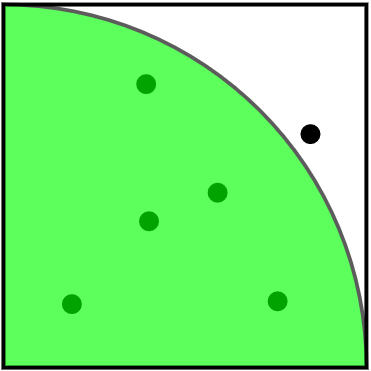
\includegraphics[scale=0.3]{Img/qCirc.png}
\end{figure}
Una volta generati i punti e valutati se ricadono all interno del primo quadrante del cerchio il calcolo del valore del pigreco è facile: \\

\vspace{1cm}
$ \pi = 4 * \frac{Punti interni alla circonferenza}{Numero di ounti generati} $ 

\lstinputlisting[language=C,  style = Cstyle,  caption = {Funzione per il calcolo del pigreco con il metodo di Monte Carlo}, label = {Code:MonteCarloPi}]{PorzioniCodice/MonteCarloPi/MCPi.c}	

Inseguito vengono riportate le tabelle che rappresentano il tempo di esecuzione e il valore calcolato.

\begin{table}[h]
\begin{tabular}{| l | c | c | c | c | c | c | c  | c |}
\hline
             & 1          & 2          & 3          & 4          & 5          & T.EXE Totale & MEDIA      & DEV.STD  \\ \hline
10\textasciicircum{}1  & 0,000008   & 0,000008   & 0,000006   & 0,000005   & 0,000006   & 0,000033     & 0,000007   & 0,000001 \\ \hline
10\textasciicircum{}2  & 0,000019   & 0,000019   & 0,000018   & 0,000018   & 0,000018   & 0,000092     & 0,000018   & 0,000001 \\ \hline
10\textasciicircum{}3  & 0,000141   & 0,000140   & 0,000141   & 0,000140   & 0,000140   & 0,000702     & 0,000140   & 0,000001 \\ \hline
10\textasciicircum{}4  & 0,001467   & 0,001501   & 0,001524   & 0,001362   & 0,001382   & 0,007236     & 0,001447   & 0,000072 \\ \hline
10\textasciicircum{}5  & 0,014029   & 0,014082   & 0,013851   & 0,013994   & 0,013971   & 0,069927     & 0,013985   & 0,000086 \\ \hline
10\textasciicircum{}6  & 0,138878   & 0,138625   & 0,138920   & 0,138916   & 0,138660   & 0,693999     & 0,138800   & 0,000145 \\ \hline
10\textasciicircum{}7  & 1,393739   & 1,387346   & 1,387775   & 1,387397   & 1,390657   & 6,946914     & 1,389383   & 0,002796 \\ \hline
10\textasciicircum{}8  & 13,881088  & 13,880401  & 13,882388  & 13,880326  & 13,880459  & 69,404662    & 13,880932  & 0,000869 \\ \hline
10\textasciicircum{}9  & 138,820115 & 138,830064 & 138,831942 & 138,863054 & 138,809745 & 694,154920   & 138,830984 & 0,019997 \\ \hline
10\textasciicircum{}10 & 195,756279 & 195,752334 & 195,733842 & 195,746235 & 195,755829 & 978,744519   & 195,748904 & 0,009329 \\ \hline
\end{tabular}
\caption{Tempi di esecuzione dell algoritmo}
\label{Tab:TimeExceMCPi}
\end{table}


\begin{table}[h]
\begin{tabular}{|l|c|c|c|c|c|c|c|}
\hline
               & 1        & 2        & 3        & 4        & 5        & MEDIA    & DEV.STD  \\ \hline
10\textasciicircum{}1  & 3,600000 & 3,200000 & 2,400000 & 3,200000 & 3,200000 & 3,120000 & 0,438178 \\ \hline
10\textasciicircum{}2  & 2,840000 & 3,160000 & 3,040000 & 3,160000 & 3,000000 & 3,040000 & 0,132665 \\ \hline
10\textasciicircum{}3  & 3,100000 & 3,136000 & 3,236000 & 3,168000 & 3,192000 & 3,166400 & 0,052046 \\ \hline
10\textasciicircum{}4  & 3,160000 & 3,128000 & 3,157200 & 3,110400 & 3,156400 & 3,142400 & 0,022114 \\ \hline
10\textasciicircum{}5  & 3,134120 & 3,138920 & 3,145400 & 3,143120 & 3,143200 & 3,140952 & 0,004482 \\ \hline
10\textasciicircum{}6  & 3,140340 & 3,140840 & 3,145420 & 3,139996 & 3,143304 & 3,141980 & 0,002319 \\ \hline
10\textasciicircum{}7  & 3,142072 & 3,141478 & 3,142091 & 3,141413 & 3,141392 & 3,141689 & 0,000360 \\ \hline
10\textasciicircum{}8  & 3,141343 & 3,141380 & 3,141467 & 3,141383 & 3,141244 & 3,141363 & 0,000081 \\ \hline
10\textasciicircum{}9  & 3,141499 & 3,141617 & 3,141583 & 3,141508 & 3,141531 & 3,141548 & 0,000051 \\ \hline
10\textasciicircum{}10 & 3,141637 & 3,141616 & 3,141607 & 3,141607 & 3,141506 & 3,141595 & 0,000051 \\ \hline
\end{tabular}
\caption{Valori calcolati}
\label{Tab:ValueMCPi}
\end{table}

Le tabelle \ref{Tab:TimeExceMCPi} e \ref{Tab:ValueMCPi} mostrano i risultati in termini di valori calcolati e il tempo di esecuzione. Le colonne 1,2,3,4,5 indicano il valore dell i-esima prova mentre ogni riga identifica il numero di punti generati.

\section{Sorting}
Gli algoritmi di ordinamento sono una parte importante dell'elaborazione dei dati e sono ampiamente utilizzati in molti aspetti, ad esempio in crittografia e nella ricerca di informazioni. Esistono molti tipi di algoritmi di ordinamento e ognuno ha i suoi vantaggi e limiti. In informatica, l'algoritmo di ordinamento è solitamente classificato come segue.

\begin{itemize}
	\item La complessità temporale.  Si basano su quanti valori si ha da distribuire. Questi vengono indicati con n.Possiamo avere una prestazione buona come $\mathcal{O}(n\log{}n)$ oppure peggiori come $\mathcal{O}(n!)$.
	\item Memoria utilizzata.
	\item Stabilita ovvero se viene preservato l'ordine relativo dei dati con chiavi uguali all'interno dei valori da ordinare.
\end{itemize}

In base alle proprietà dei diversi tipi di dati, l'efficienza può essere migliorata scegliendo algoritmi di ordinamento appropriati. In questo capitolo verranno descritti quattro algoritmi di ordinamento e verranno analizzati comparandoli all esecuzione su raspberry. L'ordinamento a cui si fa riferimento nelle sezioni successive è un ordinamento di array da mettere in ordine non decrescente.

\subsection{Bubble sort}
Bubble sort è un semplice algoritmo di ordinamento. 
L'algoritmo funziona nel modo seguente:
\begin{itemize}
	\item Confronta gli elementi adiacenti, se il primo è maggiore del secondo, scambialo.
	\item Fai lo stesso confronto di prima dalla prima coppia all'ultima coppia. 
	\item Ripeti i 2 passaggi precedenti per tutti gli elementi tranne l'ultimo.
	\item Ripeti tutti i 3 passaggi precedenti finché non sono necessari elementi da scambiare.
\end{itemize}
L'efficienza dell algoritmo è basata sull' ordinamento dell array da ordinare. Nel caso migliore l'array è gia ordinato e , passandolo all algoritmo, esegue solo il punto 1 dall inizio alla fine. In contrario il caso peggiore è quando l'array si trova nell ordine non crescente.
\begin{table}[h]
	\centering
	\begin{tabular}{lc}
              & Complessità \\
Caso peggiore &       $ \mathcal{O}(n^2)$      \\
Caso migliore &           $ \mathcal{O}(n)$   \\
\end{tabular}
	\caption{complessita bubble sort}
	\label{Tab:CompBubbleSort}
\end{table}
\\
Di seguito viene riportato il codice (Code \ref{Code:BubbleSort}) dell'algoritmo e i tempi di esecuzione(Tab \ref{Tab:Tempi esecuzione Bubblesort}) secondo la dimensione dell array e la situazione iniziale dell array:
\lstinputlisting[language=C,  style = Cstyle,  caption = {Algoritmo bubble sort scritto in c}, label = {Code:BubbleSort}]{PorzioniCodice/Sorting/Bubble.c}	

\begin{table}[h]
\centering
\begin{tabular}{| l | l | l | l |}
\hline
      & Caso peggiore & Caso migliore & Caso Generale \\ \hline
500   & 0.009426      & 0.004667      & 0.007156      \\ \hline
1000  & 0.037558      & 0.018877      & 0.028745      \\ \hline
5000  & 0.941429      & 0.470478      & 0.718178      \\ \hline
10000 & 3.784664      & 1.893387      & 2.889989      \\ \hline
20000 & 15.249109     & 7.639312      & 11.617705     \\ \hline
35000 & 46.744558     & 23.460390     & 35.640101     \\ \hline
50000 & 95.389578     & 47.888541     & 72.735791    \\ \hline
\end{tabular}
\caption{Tempi di esecuzione bubble sort}
\label{Tab:Tempi esecuzione Bubblesort}
\end{table}

\newpage
\subsection{Insertion sort}
L'arlogitmo consiste nel considerare un elemento alla volta, inserendo ciascuno nella posizione corretta tra gli elementi che sono stati ordinati. 
\begin{table}[h]
	\centering
	\begin{tabular}{lc}
              & Complessità \\
Caso peggiore &       $ \mathcal{O}(n!)$      \\
Caso migliore &           $ \mathcal{O}(n)$   \\
Caso medio &  $ \mathcal{O}(n!)$\\
\end{tabular}
	\caption{complessita insertion sort}
	\label{Tab:CompInsertionSort}
\end{table}


\lstinputlisting[language=C,  style = Cstyle,  caption = {Algoritmo bubble sort scritto in c}, label = {Code:InsertionSort}]{PorzioniCodice/Sorting/Insertion.c}	

Come nel caso del bubble sort è riportato anche il tempo di esecuzione nel caso peggiore e migliore.

\begin{table}[h]
\centering
\begin{tabular}{| l | l | l | l |}
\hline
           & Caso peggiore & Caso migliore & Caso Generale \\ \hline
500   & 0.005423      & 0.000028      & 0.002634      \\ \hline
1000  & 0.020836	    & 0.000055      & 0.010575      \\ \hline
5000  & 0.521686      & 0.000287     & 0.260862     \\ \hline
10000 & 2.103697      & 0.000645     & 1.048553      \\ \hline
20000 & 8.497346     & 0.001114      & 4.220421     \\ \hline
35000 & 26.066370     & 0.001928     & 12.969309     \\ \hline
50000 & 53.187672     & 0.002720   & 26.499820    \\ \hline

\end{tabular}
\caption{Tempi di esecuzione insertion sort}
\label{Tab:Tempi esecuzione InsertionSort}
\end{table}


\subsection{QuickSort}
L'algoritmo quicksort è un algoritmo ricorsivo del tipo divide et impera.L'algoritmo si basa:
\begin{itemize}
\item Scegli un pivot dagli elementi dell'array.
\item Ordina l' array.Se l'elemento è più grande del pivot, allora mettilo  dopo il pivot, altrimenti prima.
\item Ripetere questi due passaggi per i sottoarray finché ogni elemento non è nell'ordine corretto.
\end{itemize}

Il tempo di esecuzione nel caso peggiore di $\mathcal{O}(n!) $, il tempo di esecuzione medio di quicksort è $\mathcal{O}(n * \log{}n) $. In seguito viene mostrato l'implementazione 

\lstinputlisting[language=C,  style = Cstyle,  caption = {Algoritmo quick sort scritto in c}, label = {Code:QuickSort}]{PorzioniCodice/Sorting/Quick.c}	

\begin{table}[h]
\centering
\begin{tabular}{| l | l  |}
\hline
            & Tempo \\ \hline
500   & 0.000273      \\ \hline
1000  & 0.000610      \\ \hline
5000  & 0.003813     \\ \hline
10000 & 0.008423      \\ \hline
20000 & 0.017266     \\ \hline
35000 & 0.032285     \\ \hline
50000 & 0.048096    \\ \hline

\end{tabular}
\caption{Tempi di esecuzione quick sort}
\label{Tab:Tempi esecuzione QuickSort}
\end{table}

\subsection{Heap sort}
L'heapsort è un algoritmo di ordinamento iterativo l'implementazione utilizzata è in-place.
\todo{info algo}

\lstinputlisting[language=C,  style = Cstyle,  caption = {Algoritmo heap sort scritto in c}, label = {Code:HeapSort}]{PorzioniCodice/Sorting/Heap.c}	

\begin{table}[h]
\centering
\begin{tabular}{| l | l  |}
\hline
            & Tempo \\ \hline
500   & 0.000569      \\ \hline
1000  & 0.001272      \\ \hline
5000  & 0.008016     \\ \hline
10000 & 0.017815      \\ \hline
20000 & 0.041886     \\ \hline
35000 & 0.083366     \\ \hline
50000 & 0.128863    \\ \hline

\end{tabular}
\caption{Tempi di esecuzione heap sort}
\label{Tab:Tempi esecuzione HeapSort}
\end{table}

Come mostrato dai grafici \ref{Fig:AllSort} i risultati mostrano che il peggior algoritmo è il bubblesort mentre il migliore è quicksort.  Risultato poco notevole, nella sezione successiva un confronto più significativo.

\begin{figure}[htbp]
     \centering
     \begin{subfigure}[t]{0.45\textwidth}
         \centering
         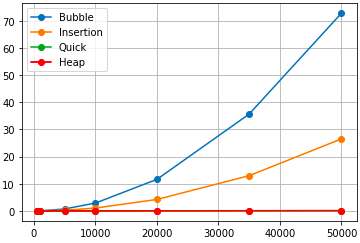
\includegraphics[width=\textwidth]{Img/GraficiSorting/AllSorting.png}
         \caption{Bubblesort insertionsort, heapsort e quicksort}
         \label{Fig:AllSortingAlg}
     \end{subfigure}
     \hfill
     \begin{subfigure}[t]{0.45\textwidth}
         \centering
         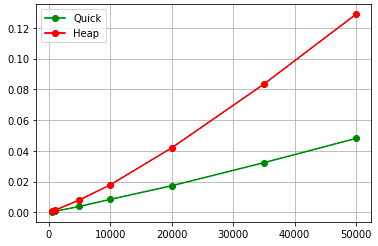
\includegraphics[width=\textwidth]{Img/GraficiSorting/QHSorting.png}
         \caption{Quicksort e Heapsort}
         \label{Fig:QHSort}
     \end{subfigure}

   \caption{Algoritmi di oridinamento a confronto}
   \label{Fig:AllSort}
\end{figure}


\subsection{Confronto Sorting}
In questa sezione vengono visualizzati i risultati a confronto. Per prima cosa iniziamo con confrontare i risultati con l'esecuzione su MacBook.

\begin{figure}[htbp]
     \centering
     \begin{subfigure}[t]{0.49\textwidth}
         \centering
         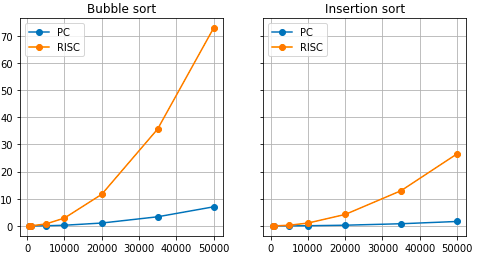
\includegraphics[width=\textwidth]{Img/GraficiSorting/BubbleInsert.png}
       
     \end{subfigure}
     \hfill
     \begin{subfigure}[t]{0.49\textwidth}
         \centering
         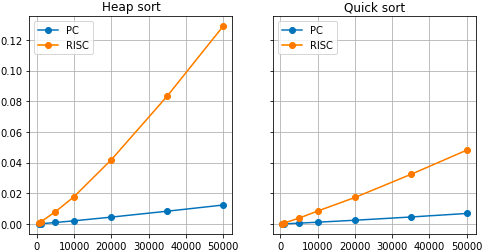
\includegraphics[width=\textwidth]{Img/GraficiSorting/HeapQuick.png}
        
     \end{subfigure}

   \caption{Algoritmi di oridinamento a confronto eseguiti su PC e su RISC-V}
   \label{Fig:AllSort_PC}
\end{figure}
	
	
	\begin{table}[h]
		\centering
		\begin{tabular}		{| l | c | c | c | c |}
		\hline
		      & Bubblesort & Insertionsort & Heapsort & Quicksort \\ \hline
500   & 0.000491      & 0.000196      & 0.000057 & 0.000052     \\ \hline
1000  & 0.001871	    & 0.000723      & 0.000145 & 0.000080     \\ \hline
5000  & 0.055505      & 0.016859     & 0.000975  & 0.000544   \\ \hline
10000 & 0.247916      & 0.066411     & 0.002083 & 0.001164     \\ \hline
20000 & 1.056383   & 0.261627      & 0.004485  & 0.002441   \\ \hline
35000 & 3.359662     & 0.800075     & 0.008340  & ;0.004557   \\ \hline
50000 & 7.019640     & 1.633171   & 0.012359  & 0.006857  \\ \hline

		\end{tabular}
		\caption{Tempi di esecuzione degli algoritmi di sorting su PC}
		\label{Fig:PcSort}
	\end{table}

La tabella \ref{Fig:PcSort} mostra i tempi di esecuzione degli algoritmi di ordinamento. Confrontando i tempi del PC e si nota che in generale si ha, circa, un ordine di grandezza di differenza ricordando i 2.2 GHz del processore e 8Gb da 1600MHz del MacBook confrontati con il processore da 1 GHz con memoria da 2Gb a 1333 MHz vengono tradotti in un miglior tempo di esecuzione di un fattore 10.
Un altro confronto lo possiamo fare con raspberry pi \footnote{Il modello utilizzato è il modello Raspberry model B mostrato in figura \ref{Fig:RBmodelB} }.

\begin{figure}[h]
\centering
	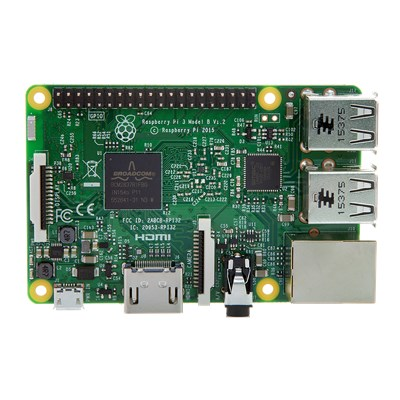
\includegraphics[scale=0.5]{RBTop.jpeg}
	\label{Fig:RBmodelB}
	\caption{Vista superiore Raspberry model B}
\end{figure}

Il Raspberry Pi utilizzato è Raspberry Pi model B. La board datata 2013 è stata sviluppata come board scolastica e successivamente applicata a molti contesti come nel mondo embedded.
Con la dimensione di una carta di credito il Raspberry ha una RAM di 512 MB e una CPU da 700 MHz,due porte USB (Universal Serial Bus) e un'Ethernet da 100 MB porta. In aggiunta a ciò, ci sono pin di input/output (GPIO) per uso generico per collegare alcuni hardware.  La tabella \ref{Tab:RaspSorting} mostra i tempi di esecuzione degli algoritmi di ordinamento eseguiti su Raspberry.

\begin{table}[h]
		\centering
		\begin{tabular}		{| l | c | c | c | c |}
		\hline
		      & Bubblesort & Insertionsort & Heapsort & Quicksort \\ \hline
500   & 0.020337      & 0.004877      & 0.000825 & 0.000511     \\ \hline
1000  & 0.078527	    & 0.020353      & 0.001894 & 0.001141     \\ \hline
5000  & 2.030446      & 0.045018     & 0.013863  & 0.009072   \\ \hline
10000 & 8.535436      & 1.874295     & 0.027671 & 0.018542     \\ \hline
20000 & 34.733894   & 7.842624      & 0.058596  & 0.038194   \\ \hline
35000 & 117.622606     & 24.076289     & 0.114716  & 0.082891   \\ \hline
50000 & 250.008917     & 51.757841   & 0.210807  & 0.157344  \\ \hline

		\end{tabular}
		\caption{Tempi di esecuzione Raspberry Pi B}
		\label{Tab:RaspSorting}
			\end{table}

\begin{figure}[htbp]
     \centering
     \begin{subfigure}[t]{0.49\textwidth}
         \centering
         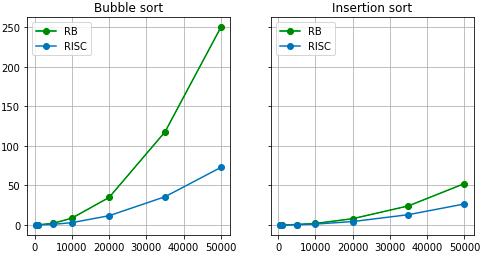
\includegraphics[width=\textwidth]{Img/GraficiSorting/BISort_RB.png}
        
     \end{subfigure}
     \hfill
     \begin{subfigure}[t]{0.49\textwidth}
         \centering
         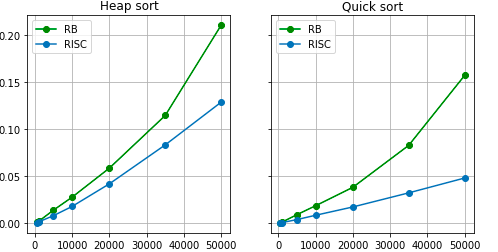
\includegraphics[width=\textwidth]{Img/GraficiSorting/HQSort_RB.png}
         
     \end{subfigure}

   \caption{Algoritmi di oridinamento a confronto eseguiti su Raspberry e su RISC-V}
   \label{Fig:AllSort_RB}
\end{figure}

I grafici \ref{Fig:AllSort_RB} mostrano i tempi di esecuzione degli algoritmi di sorting comparati tra Rasberry e RISC-V. In ogni grafico si vede che il tempo di esecuzione è migliore su RISC-V. Prendendo in considerazione il Bubblesort nel caso con 50000 elementi la board con processore RISC-V è 4 volte piu veloce del raspberry in altri casi, come ad esempio per heap sort, il miglioramente di RISC-V è 1.6 rispetto a Raspberry. Possiamo concludere che il miglioramento è dato dalla CPU e dalla memoria.  \todo{More}

\section{BackTracking}
Un altro problema che si puo affrontare è il problema del backtracking, ovvero quella tecnica per cui è necessario tornare su dei passi precedenti per trovare la soluzione al problema. Il primo programma utilizzato è un solutore di sudoku.
I primi sudoku sono di difficoltà crescente mentre gli utlimi sono impossibili, uno impossibile per costruzione (sbagliato dalla partenza) , e l'altro impossibile completarlo.
\begin{table}
\centering
\begin{tabular}{  |l | c | c |}
\hline
	& RISC-V & PC \\ \hline
	1 & 0.004475 & 0.000384  \\ \hline
2 & 0.055382 &0.004791           \\ \hline
3 & 0.000282 &0.000026  \\ \hline
4 & 0.048991 &0.005037  \\ \hline
5 & 0.297553 &0.025939  \\ \hline
6 & 1.488701 &0.122498  \\ \hline
7 & 6.548320 &0.534505  \\ \hline
8 & 0.001508 &0.000241  \\ \hline
Vuoto & 0.001680 & 0.000267  \\ \hline
\end{tabular}

	\caption{Tempi di esecuzione del solutore di sudoku}
	\label{Tab:SudoSolver}
	\end{table}
	
Il secondo problema che utilizza il backtracking è un solutore di labirinti.

\begin{table}
\centering
\begin{tabular}{  |l | c | c |}
\hline
 & RISC & PC  \\ \hline
maze0 & 0.000102 & 0.000007  \\ \hline
maze1 & 0.005261 & 0.000235  \\ \hline
maze2 &0.009123 & 0.000371  \\ \hline
\end{tabular}

	\caption{Tempi di esecuzione del solutore di labirinti}
	\label{Tab:MazeSolver}
	\end{table}

\todo{More}
\todo{add Reference}



\chapter{Progetti}
\todo{Rileggi/Correggi capitolo 6: Progetti \ldots}
Un progetto, con poco piu di dieci anni, ha gia ricevuto molte attenzioni da parte delle aziende. A oggi sono diverse le aziende che hanno scelto RISC-V per i loro progetti, e sembra che l'ISA sia ora pronta a fare il grande salto.  Due anni fa la statunitense Micro Magic, ha annunciato quello che ha definito "il core RISC-V a 64 bit più veloce al mondo", una soluzione che secondo loro è in grado di battere chip di ultima generazione come l'Apple M1 e le soluzioni basate su ARM.  L'azienda ha dimostrato una prototipo in grado di operare a 5 GHz. Un risultato, probabilmente, collegato a questo è che l' Apple ha deciso di tagliare i ponti con le architetture x86. La casa di Cupertino sembra che si voglia rivolgere verso l'architettura open source RISC-V. A confermarlo è un annuncio di lavoro per un \textit{"RISC-V High Performance Programmer"}.\\
Al momento non c'è nulla che indichi che  Apple sia pronta a lasciare arm per passare a RISC-V, ma probabilmente integrerà nell'ecosistema attuale qualche processore RISC-V. Anche un altra grande azienda, AMD, ha pubblicato un annuncio di lavoro per una CPU RISC-V non ben precisata. Anche nel mondo del machine learning RISC-V si fa sentire.  Recentemente è stato presentato un acceleratore per il machine learning basato su un chip RISC-V, chiamato ET-SoC-1. Il processore è  dotato di 1088 core: a bordo della scheda vi sono sei chip. ET-SoC-1 può funzionare come processore standalone o come acceleratore.Secondo il CEO  di Esperanto Technologies si tratta del chip RISC-V commerciale \textit{ "più veloce al mondo"}. \\
Tornando nel contesto domestico alcune notizie ipotizzano un laptop nominato ROMA.
Per ROMA le aziende DeepComputing e Xcalibyte hanno deciso di scommettere su  RISC-V, progettando un laptop differente rispetto ai moderni moderni. Il portatile avrà una CPU quad-core, GPU e NPU (Neural Processing Unit) per l’accelerazione 3D. Sarà equipaggiato con 256 GB di SSD e 16 GB di RAM. Supporterà la maggior parte dei sistemi Linux. Il laptop è stato pensato principalmente per gli sviluppatori che scrivono codice per architettura RISC ma nulla vieta che successivamente sarà disponibile una versione per i non programmatori.\\
Sempre in una realtà quotidiana Patrick Little, CEO di SiFive, ha dichiarato che entro il 2023 probabilmente vedremo sul mercato il primo smartphone basato su RISC-V sottolineando le enormi potenzialità dell'architettura e del design della sua azienda.



\chapter{Dibattito ARM vs RISC-V}
\todo{Rileggi/Correggi capitolo 7: Dibattito \ldots}

Quando si parla di processori una cosa importate da prendere in considerazione è ISA, quando si vuole scrivere un programma è molto utile conoscere il target per il proprio codice. Nell'ecosistema eterogeneo degli ISA i piu utilizzati sono x86 e ARM che hanno un approccio CISC e RISC rispettivamente. Le due ISA vengono applicate a sistemi ben differenti, ad esmpio il sistema sviluppato da Intel si applica a sistemi di grandi dimensione  come i sistemi HPC e i cluster mentre l'ambiente ARM viene utilizzato a sistemi ben piu piccoli. In questo contesto RISC-V, con il suo approccio RISC, sembrerebbe che voglia sostituirsi  ARM. \\
Facciamo confronto con ARM e RISC il primo è basato su un IP proprietario che viene concesso alle società con un numero relativamente contenuto di fornitori, RISC invece ha un architettura delle specifiche royalty-free e i processori sono disponibili e esistono anche core con licenza commerciale. Le community hanno dimensino differenti, piu strutturata quella di ARM che aiuta i progettisti per specifiche applicazioni, contraposta è quella di RISC , che con poco piu di 10 anni di vita la community è piu contenuta main continua crescita. ARM dispone di team di ingegneri che sviluppano sistemi hardware che rendono facile per i progettisti incorporare CPU ARM, mentre i progettisti possono sperimentare e sviluppare sistemi RISC-V gratuitamente, c’è poco o nessun supporto per la progettazione dell’hardware. Per concludere L’ISA RISC-V è organizzato in gruppi di istruzioni  e offre la possibilità di utilizzare estensioni fornendo allo standard ISA  un supporto per applicazioni specifiche. Ad esempio, l’estensione RISC-V Vector (RVV) recentemente rilasciata consente ai core del processore basati su RISC-V ISA di elaborare array di dati insieme alle tradizionali operazioni scalari, per accelerare il calcolo di singoli flussi di istruzioni su grandi insiemi di dati.  In contradizione con l'approccio iniziale di ARM che non forniva estendibilità ma solo in seguito.\\
Passiamo ora a sistemi un po piu grandi.  L'azienda E4 Computer Engineering ha progettato il suo primo Arm-based cluster nel 2012 (INSERISCI NOTE BIB).  Oggi l' E4 sta  integrando un cluster basato sul processore HiFive Unmatched (di SiFive). Questa azione inaugura una nuova era di sviluppo RISC-V basato su Linux. Il processore utilizzato è basatosu RISC-V che utilizza multi-core ad alte prestazioni, 64 bit dual-issue e superscalare.  In questo modo si fornisce l’accesso ad entrambe le architetture ARM e RISC-V, cosicchè gli utenti e sviluppatori possono testare ampiamente le loro applicazioni e codici e fornire indicazioni per trovare la migliore soluzione complessiva ai loro requisiti.

L’uso di processori RISC-V è crescente,  le grandi aziende stanno già cercando alternative ad ARM. Anche se ARM è stata acquisita da  NVIDIA,  RISC-V si fa sentire sul mercato. Alcuni dei suoi partner sono Google, Intel e Huawei o altri come Arduino, AntMicro e Oculus.  \\

Tuttavia, solo perché qualcosa è gratuito non significa che prenderà il comando. Prendiamo come esempio il sistema Linux la maggior parte delle distribuzioni sono gratuite, ma Linux costituisce una piccola percentuale dei sistemi operativi in tutto il mondo.   Con il migliorare della tecnologia il supporto a RISC-V aumenterà, grazie anche alla community, che porterà i progetisti ad avere un opzione di un architettura gratuita senza limitazioni e altamente configurabile ed estendibile ma non si ha certezza se prenderà una grossa fetta di mercato.

\chapter{Conclusione}
\textbf{DESKTOP CON PROCESSORE RISC-V SEE BIB}
%\addcontentsline{toc}{chapter}{Bibliografia}

\printbibliography

\end{document}
